\subsection{Semileptonic decays}
\label{sec:charm:semileptonic}

\subsubsection{Introduction}

Semileptonic decays of $D$ mesons involve the interaction of a leptonic
current with a hadronic current. The latter is nonperturbative
and cannot be calculated from first principles; thus it is usually
parameterized in terms of form factors. The transition matrix element 
is written
\begin{eqnarray}
  {\cal M} & = & -i\,\frac{G_F}{\sqrt{2}}\,V^{}_{cq}\,L^\mu H_\mu\,,
  \label{Melem}
\end{eqnarray}
where $G_F$ is the Fermi constant and $V^{}_{cq}$ is a CKM matrix element.
The leptonic current $L_\mu$ is evaluated directly from the lepton spinors 
and has a simple structure; this allows one to extract information about 
the form factors (in $H^{}_\mu$) from data on semileptonic decays~\cite{Becher:2005bg}.  
Conversely, because there are no final-state interactions between the
leptonic and hadronic systems, semileptonic decays for which the form 
factors can be calculated allow one to 
determine~$V^{}_{cq}$~\cite{Kobayashi:1973fv}.

\subsubsection{$D\ra P \overline \ell \nu_{\ell}$ decays}

When the final state hadron is a pseudoscalar, the hadronic 
current is given by
\begin{eqnarray}
H_\mu & = & \left< P(p) | \bar{q}\gamma^\mu c | D(p') \right> \ =\  
f_+(q^2)\left[ (p' + p)^\mu -\frac{m_D^2-m_P^2}{q^2}q^\mu\right] + 
 f_0(q^2)\frac{m_D^2-m_P^2}{q^2}q^\mu\,,
\label{eq:hadronic}
\end{eqnarray}
where $m_D$ and $p'$ are the mass and four momentum of the 
parent $D$ meson, $m_P$ and $p$ are those of the daughter meson, 
$f_+(q^2)$ and $f_0(q^2)$ are form factors, and $q = p' - p$.  
Kinematics require that $f_+(0) = f_0(0)$.
The contraction $q^\mu L_\mu$ results in terms proportional 
to $m^{}_\ell$\cite{Gilman:1989uy}, and thus for $\ell=e $
the terms proportionals to $q^\mu$ in Eq.~(\ref{eq:hadronic}) are negligible. 
Considering that only the $f_+(q^2)$ form factor 
is relevant, the differential partial width is
% integrated over various angular distributions is
\begin{eqnarray}
\frac{d\Gamma(D \to P \bar \ell \nu_\ell)}{dq^2\, d\cos\theta_\ell} & = & 
   \frac{G_F^2|V_{cq}|^2}{32\pi^3} p^{*\,3}|f_{+}(q^2)|^2\sin\theta^2_\ell\,,
\label{eq:dGamma}
\end{eqnarray}
where ${p^*}$ is the magnitude of the momentum of the final state hadron
in the $D$ rest frame.

%parameterization takes advantage of dispersion relations (see,
%{\it e.g.}, Ref.~\cite{Boyd:1994tt}), which allow expression of a form
%factor in terms of

\subsubsection{Form factor parameterizations} 

The form factor is traditionally parameterized with an explicit pole 
and a sum of effective poles:
\begin{eqnarray}
f_+(q^2) & = & \frac{f_+(0)}{(1-\alpha)}\Bigg [
\left(\frac{1}{1- q^2/m^2_{\rm pole}}\right)\ +\ 
\sum_{k=1}^{N}\frac{\rho_k}{1- q^2/(\gamma_k\,m^2_{\rm pole})}\Bigg ]\,,
\label{eqn:expansion}
\end{eqnarray}
where $\rho_k$ and $\gamma_k$ are expansion parameters. The parameter
$m_{{\rm pole}}$ is the mass of the lowest-lying $c\bar{q}$ resonance
with the appropriate quantum numbers; this is expected to provide the
largest contribution to the form factor for the $c\ra q$ transition.  
For example, for $D\to\pi$ transitions the dominant resonance is
expected to be $D^*$, and thus $m^{}_{\rm pole}=m^{}_{D^*}$.

\subsubsubsection{Simple pole}

Equation~(\ref{eqn:expansion}) can be simplified by neglecting the 
sum over effective poles, leaving only the explicit vector meson pole. 
This approximation is referred to as ``nearest pole dominance'' or 
``vector-meson dominance.''  The resulting parameterization is
\begin{eqnarray}
  f_+(q^2) & = & \frac{f_+(0)}{(1-q^2/m^2_{\rm pole})}\,. 
\label{SimplePole}
\end{eqnarray}
However, values of $m_{{\rm pole}}$ that give a good fit to the data 
do not agree with the expected vector meson masses~\cite{Hill:2006ub}. 
To address this problem, the ``modified pole'' or Becirevic-Kaidalov~(BK) 
parameterization~\cite{Becirevic:1999kt} was introduced.
$m_{\rm pole} /\sqrt{\alpha_{\rm BK}}$
is interpreted as the mass of an effective pole, higher than $m_{\rm pole}$, thus it is expected that $\alpha_{\rm BK}<1$.

 
%This parametrization assumes that gluon 
%hard-scattering contributions ($\delta$) are near zero, and scaling
%violations ($\beta$) are near unity~\cite{Hill:2006ub}:
%\begin{eqnarray}
%1 + 1\slash \beta - \delta & \equiv & 
%\frac{\left(m_D^2 - m_{P}^2\right)}{f_+(0)}\ 
%\left.\frac{df_+}{dq^2}\right|_{q^2=0}\ \approx\ 2\,.
%\end{eqnarray}

The parameterization takes the form
\begin{eqnarray}
f_+(q^2) & = & \frac{f_+(0)}{(1-q^2/m^2_{\rm pole})}
\frac{1}{\left(1-\alpha^{}_{\rm BK}\frac{q^2}{m^2_{\rm pole}}\right)}\,.
\end{eqnarray}
 
%To be consistent with $1 + 1\slash \beta - \delta\approx 2$, the 
%parameter $\alpha^{}_{\rm BK}$ should be near the value~1.75.

This parameterization has been used by several experiments to 
determine form factor parameters.
Measured values of $m^{}_{\rm pole}$ and $\alpha^{}_{\rm BK}$ are
listed Tables~\ref{kPseudoPole} and~\ref{piPseudoPole} for
$D\to K\ell\nu_{\ell}$ and $D\to\pi\ell\nu_{\ell}$ decays, respectively.
%These values are plotted in Figs.~\ref{Kpole} and~\ref{pipole}.
%Both tables show $\alpha^{}_{BK}$ to be substantially lower than
%the expected value of~$\sim$\,1.75.

%As is clear from the figures, the $K\ell\nu$ data yield pole masses that
%are significantly lower than the mass of the $D_s^*$ resonance that
%should dominate in the vector dominance (simple pole) model.  The
%$\pi\ell\nu_{\ell}$ data also show a trend toward a pole mass lower than the
%physical $D^*$ pole mass, with the recent CLEO-c measurement showing a
%significant discrepancy. The simple pole parameterization can typically
%provide a good fit to the data.  However, the unphysically low mass
%parameters indicate that higher mass resonances and the $DK$ and $D\pi$
%continuum contribute non-negligibly to the decay process.

\subsubsubsection{$z$ expansion}

An alternative series expansion around some value $q^2=t_0$ to parameterize 
$f^{}_+$ can be used~\cite{Boyd:1994tt,Boyd:1997qw,Arnesen:2005ez,Becher:2005bg}. This parameterization is model 
independent and satisfies general QCD constraints, being suitable for fitting experimental data.
The expansion is given in terms of a complex parameter $z$,
which is the analytic continuation of $q^2$ into the complex plane:
\begin{eqnarray}
z(q^2,t_0) & = & \frac{\sqrt{t_+ - q^2} - \sqrt{t_+ - t_0}}{\sqrt{t_+ - q^2}
	  + \sqrt{t_+ - t_0}}\,, 
\end{eqnarray}
where $t_\pm \equiv (m_D \pm m_P)^2$ and $t_0$ is the (arbitrary) $q^2$ 
value corresponding to $z=0$. The physical region corresponds to $\pm|z|_{max} = \pm 0.051$ 
for $D\to K \ell \nu_\ell$ and $= \pm 0.17$ for  $D\to \pi \ell \nu_\ell$, 
using $t_{0}= t_{+} (1-\sqrt{1-t_{-}/t_{+}})$.  

The form factor is expressed as
\begin{eqnarray}
f_+(q^2) & = & \frac{1}{P(q^2)\,\phi(q^2,t_0)}\sum_{k=0}^\infty
a_k(t_0)[z(q^2,t_0)]^k\,,
\label{z_expansion}
\end{eqnarray}
where the $P(q^2)$ factor accommodates sub-threshold resonances via
\begin{eqnarray}
P(q^2) & \equiv & 
\begin{cases} 
1 & (D\to \pi) \\
z(q^2,M^2_{D^*_s}) & (D\to K)\,. 
\end{cases}
\end{eqnarray}
The ``outer'' function $\phi(t,t_0)$ can be any analytic function,
but a preferred choice (see, {\it e.g.}
Refs.~\cite{Boyd:1994tt,Boyd:1997qw,Bourrely:1980gp}) obtained
from the Operator Product Expansion (OPE) is
\begin{eqnarray}
\phi(q^2,t_0) & =  & \alpha 
\left(\sqrt{t_+ - q^2}+\sqrt{t_+ - t_0}\right) \times  \nonumber \\
 & & \hskip0.20in \frac{t_+ - q^2}{(t_+ - t_0)^{1/4}}\  
\frac{(\sqrt{t_+ - q^2}\ +\ \sqrt{t_+ - t_-})^{3/2}}
     {(\sqrt{t_+ - q^2}+\sqrt{t_+})^5}\,,
\label{eqn:outer}
\end{eqnarray}
with $\alpha = \sqrt{\pi m_c^2/3}$.
The OPE analysis provides a constraint upon the 
expansion coefficients, $\sum_{k=0}^{N}a_k^2 \leq 1$.
These coefficients receive $1/M_D$ corrections, and thus
the constraint is only approximate. However, the
expansion is expected to converge rapidly since 
$|z|<0.051\ (0.17)$ for $D\ra K$ ($D\ra\pi$) over 
the entire physical $q^2$ range, and Eq.~(\ref{z_expansion}) 
remains a useful parameterization. The main disadvantage as compared to 
phenomenological approaches is that there is no physical interpretation 
of the fitted coefficients $a_K$.

\subsubsubsection{Three-pole formalism}
A recent update of the vector pole dominance model has been developed for the $D \to \pi \ell \nu_\ell$ channel~\cite{Becirevic:2014kaa}.
It uses information of the residues of the semileptonic form factor at its first two poles, the $D^\ast$ 
and $D^{\ast '}$ resonances.  
The form factor is expressed as an infinite sum of $J^P =1^-$ states with masses $m_{D^\ast_n}$: 
\begin{eqnarray}
f_+(q^2) = \sum_{n=0}^\infty { \; \displaystyle{\underset{q^2= m_{D^\ast_n}^2}{\rm Res}} f_+(q^2)\;\over m_{D^\ast_n}^2-q^2} \,,
\label{ThreePole}
\end{eqnarray}
with the residues given by 
\begin{eqnarray}
\displaystyle{\underset{q^2=m_{D_n^\ast}^2}{\rm Res}} f_+(q^2)= {1\over 2} m_{D_n^\ast} f_{D_n^\ast} g_{D_n^\ast D\pi}\,, 
\label{Residua}
\end{eqnarray}
Values of the $f_{D^\ast}$ and $f_{D^{\ast '}}$ decay constants have been obtained by Lattice QCD calculations, 
relative to $f_{D}$, with 2$\%$ and 28$\%$ precision, respectively \cite{Becirevic:2014kaa}. 
The couplings to the $D\pi$ state, $g_{D^\ast D\pi}$ and $g_{D^{\ast '} D\pi}$, are extracted from the accurate 
measurements of the $D^\ast$ and  $D^{\ast '}$ widths by \babar~\cite{Lees:2013uxa,delAmoSanchez:2010vq} and LHCb~\cite{Aaij:2013sza} experiments. 
Thus the contribution from the first pole is known with a $3\%$ accuracy. 
The contribution from the $D^{\ast '}$ is determined with poorer accuracy, $\sim 30\%$, mainly due to lattice uncertainties.   

A {\it superconvergence} condition is applied \cite{Burdman:1996kr}: 
\begin{eqnarray}
\sum_{n=0}^\infty { \; \displaystyle{\underset{q^2=m_{D^\ast_n}^2}{\rm Res}} f_+(q^2) }= 0 \,,
\label{superconvergence}
\end{eqnarray}
protecting the form factor behavior at large $q^2$.
Within this model the first two poles are not enough to describe the data, and a third effective pole has to be included. 

One of the advantages of this phenomenological model 
is that it can be extrapolated outside the charm physical region, providing a method to 
extract the CKM matrix element $V_{ub}$ using the relation between the form factors of the 
$D\to \pi\ell \nu$ and $B\to \pi\ell \nu$ decay channels. It will be used once Lattice calculations provide
the form factor ratio $f^{+}_{B\pi}(q^2)/f^{+}_{D\pi}(q^2)$ at the same pion energy. 

\subsubsection{Experimental techniques and results}
 Different techniques by several experiments have been used to measure $D$ meson semileptonic decays with a 
pseudoscalar particle in the final state. The most recent results are provided by the \babar and BES III collaborations.
They have been presented at the ICHEP 2014 conference and are preliminary.  
Belle \cite{Widhalm:2006wz}, \babar \cite{Aubert:2007wg} and CLEO-c \cite{Besson:2009uv,Dobbs:2007aa} 
collaborations have previously reported results. 
%The BES III experiment has also reported preliminary results at the CHARM 2012 conference with 923 $\pb^{-1}$ \cite{BESIII}.  
The Belle collaboration fully reconstructs the $D$ events from the continuum under the $\Upsilon(4S)$ resonance, 
achieving a very good $q^2$ resolution ($\Delta q^2 = 15 MeV^2$) and low background level, 
but having a low efficiency. Using 282~$\fb^{-1}$, about 1300 and 115 signal semileptonic decays are 
isolated for each lepton flavor (e and $\mu$), respectively. 
The \babar experiment uses a partial reconstruction technique where the semileptonic decays are tagged 
through the $ D^{\ast +}\to D^0\pi^+$ decay. 
The $D$ direction and neutrino energy is obtained using information of the rest of the event. 
With 75~$\fb^{-1}$ 74000 signal events in the $D^0 \to {K}^- e^+ \nu$ mode are obtained. 
This technique provides larger statistics but higher background level and poorer $q^2$ resolution ($\Delta q^2$ ranges from 66 to 219 $MeV^2$). In this case the measurement of the branching fraction is obtained by normalizing to the $D^0 \to K^- \pi^+$ decay channel and can benefit from future improvements in the determination of this reference channel. The measurement of the Cabibbo suppressed mode has been recently obtained 
using the same technique and 350~fb$^{-1}$ data. 5000 $D^0 \to {\pi}^- e^+ \nu$ signal events are reconstructed using this method \cite{babar-new}.  
The CLEO-c experiment uses two different methods to measure charm semileptonic decays. 
Tagged analyses \cite{Besson:2009uv} rely on the full reconstruction of $\psi(3770)\to D {\overline D}$ events. One of the D mesons is reconstructed in a hadronic decay mode, the other in the semileptonic channel. The only missing particle is the neutrino so the $q^2$ resolution is very good and the background level very low.   
With the entire CLEO-c data sample, 818 $\pb^{-1}$, 14123 and 1374 signal events are reconstructed for 
the $D^0 \to K^{-} e^+\nu$ and $D^0\to \pi^{-} e^+\nu$ channels, and 8467 and 838 for the 
$D^+\to {\overline K}^{0} e^+\nu$ and $D^+\to \pi^{0} e^+\nu$ decays, respectively. 
Another technique without tagging the D meson in a hadronic mode (``untagged'' in the following) has been also 
used by CLEO-c \cite{Dobbs:2007aa}. This method rests upon the association of the missing energy and momentum in 
an event with the neutrino four momentum, with the penalty of larger background as compared to the tagged method. 
Using the ``tagged'' method the BES III experiment has measured the $D^0 \to {K}^- e^+ \nu$ and 
$D^0 \to {\pi}^- e^+ \nu$ decay channels. With 2.9~fb$^{-1}$ they fully reconstruct 70700 and 6300 signal 
events for each channel, respectively. These results are preliminary. 

  Previous measurements were also performed by CLEO~III and FOCUS experiments. 
Events registered at the $\Upsilon (4S)$ energy corresponding to an integrated luminosity of 7 $\fb^{-1}$ were 
analyzed by CLEO~III \cite{Huang:2004fra}. 
In the FOCUS fixed target photo-production experiment $D^0$ semileptonic events were obtained from the decay of 
a $D^{\ast +}$, and the kaon or pion was reconstructed in the muon channel. 
%The $q^2$ resolution is 0.22 $GeV^2$. 
%They reconstructed 12840 signal events were obtained for the $\D^0 \to K^- \mu^+ \nu$ chnnel and 

 Results of the hadronic form factor parameters by the different groups are given in Tables
\ref{kPseudoPole} and \ref{piPseudoPole} for $m_{pole}$ and $\alpha_{BK}$. 
\begin{table}[htbp]
\caption{Results for $m_{\rm pole}$ and $\alpha_{\rm BK}$ from various
  experiments for $D^0\to K^-\ell^+\nu$ and $D^+\to K_S\ell^+\nu$
  decays. 
%The last entry is a lattice QCD prediction (errors have been increased as compared to the publication 
%to take into account remaining systematic uncertainties in Lattice calculations, as advised by the authors).
\label{kPseudoPole}}
\begin{center}
\begin{tabular}{cccc}
\hline
\vspace*{-10pt} & \\
 $D\to K\ell\nu_\ell$ Expt. & Ref.  & $m_{\rm pole}$ (GeV$/c^2$) 
& $\alpha^{}_{\rm BK}$       \\
\vspace*{-10pt} & \\
\hline
 \omit        & \omit                         & \omit                                  & \omit                  \\
 CLEO III     & \cite{Huang:2004fra}          & $1.89\pm0.05^{+0.04}_{-0.03}$          & $0.36\pm0.10^{+0.03}_{-0.07}$ \\
 FOCUS        & \cite{Link:2004dh}            & $1.93\pm0.05\pm0.03$                   & $0.28\pm0.08\pm0.07$     \\
 Belle        & \cite{Widhalm:2006wz}         & $1.82\pm0.04\pm0.03$                   & $0.52\pm0.08\pm0.06$     \\
 \babar        & \cite{Aubert:2007wg}          & $1.889\pm0.012\pm0.015$                & $0.366\pm0.023\pm0.029$  \\

 CLEO-c (tagged)   &\cite{Besson:2009uv}      & $1.93\pm0.02\pm0.01$                   & $0.30\pm0.03\pm0.01$     \\
 CLEO-c (untagged, $D^0$) &\cite{Dobbs:2007aa}       & $1.97 \pm0.03 \pm 0.01 $ & $0.21 \pm 0.05 \pm 0.03 $  \\
 CLEO-c (untagged, $D^+$) &\cite{Dobbs:2007aa}       & $1.96 \pm0.04 \pm 0.02 $ & $0.22 \pm 0.08 \pm 0.03$  \\
% BESIII (prel)     &\cite{BESIII}                     & $1.943 \pm 0.025 \pm 0.003$ & $ 0.265 \pm 0.045 \pm 0.006$   \\ 0.923/fb
  BESIII (preliminary)     &\cite{BESIII-new}                & $1.921 \pm 0.010 \pm 0.007$ & $ 0.309 \pm 0.020 \pm 0.013$   \\ %3/fb

% CLEO-c ($D^0\to K^+$) & \cite{GaoICHEP06}    & $1.943^{+0.037}_{-0.033}\pm 0.011$ & $0.258^{+0.063}_{-0.065}\pm0.020$  \\
% CLEO-c ($D^0\to K^+$) & \cite{Dobbs:2007sm}  & $1.97\pm 0.03\pm 0.01$                 & $0.21\pm0.05\pm0.03$                  \\
% CLEO-c ($D^+\to K_S$) & \cite{GaoICHEP06}    & $2.02^{+0.07}_{-0.06}\pm 0.02$     & $0.127^{+0.099}_{-0.104}\pm0.031$  \\
% CLEO-c ($D^+\to K_S$) & \cite{Dobbs:2007sm}  & $1.96\pm 0.04\pm 0.02$                 & $0.22\pm0.08\pm0.03$                  \\
%\hline
% Fermilab lattice/MILC/HPQCD & \cite{Aubin:2004ej}            & --                                &  $0.50\pm0.04\pm0.07$         \\
\vspace*{-10pt} & \\
\hline
\end{tabular}
\end{center}
\end{table}

\begin{table}[htbp]
\caption{Results for $m_{\rm pole}$ and
  $\alpha_{\rm BK}$ from various experiments for 
  $D^0\to \pi^-\ell^+\nu$ and $D^+\to \pi^0\ell^+\nu$ decays.  
%The last entry is a lattice QCD prediction (errors have been increased as compared to the publication 
%to take into account remaining systematic uncertainties in Lattice calculations, as advised by the authors).
\label{piPseudoPole}}
\begin{center}
\begin{tabular}{cccc}
\hline
\vspace*{-10pt} & \\
 $D\to \pi\ell\nu_\ell$ Expt. & Ref.               & $m_{\rm pole}$ (GeV$/c^2$) & $\alpha_{\rm BK}$ \\
\vspace*{-10pt} & \\
\hline
 \omit        & \omit                         & \omit                                  & \omit                  \\
 CLEO III     & \cite{Huang:2004fra}          & $1.86^{+0.10+0.07}_{-0.06-0.03}$       & $0.37^{+0.20}_{-0.31}\pm0.15$         \\
 FOCUS        & \cite{Link:2004dh}            & $1.91^{+0.30}_{-0.15}\pm0.07$          & --                                    \\
 Belle        & \cite{Widhalm:2006wz}         & $1.97\pm0.08\pm0.04$                   & $0.10\pm0.21\pm0.10$                  \\
 CLEO-c (tagged)   &\cite{Besson:2009uv}      & $1.91\pm0.02\pm0.01$                   & $0.21\pm0.07\pm0.02$     \\
 CLEO-c (untagged, $D^0$) &\cite{Dobbs:2007aa}       & $1.87 \pm0.03 \pm 0.01 $ & $0.37 \pm 0.08 \pm 0.03$  \\
 CLEO-c (untagged, $D^+$) &\cite{Dobbs:2007aa}       & $1.97 \pm0.07 \pm 0.02 $ & $0.14 \pm 0.16 \pm 0.04$  \\
% BESIII (prel)     &\cite{BESIII}                    & $1.876 \pm 0.023 \pm 0.004$ & $ 0.315 \pm 0.071 \pm 0.012$   \\ 0.9/fb
 BES III (preliminary)     &\cite{BESIII-new}                & $1.911 \pm 0.012 \pm 0.004$ & $ 0.279 \pm 0.035 \pm 0.011$   \\ %3/fb
  \babar (preliminary)     &\cite{babar-new}                & $1.906 \pm 0.029 \pm 0.023$ & $ 0.268 \pm 0.074 \pm 0.059$   \\

% CLEO-c ($D^0\to\pi^+$) & \cite{GaoICHEP06}   & $1.941^{+0.042}_{-0.034}\pm0.009$ & $0.20^{+0.10}_{-0.11}\pm0.03$  \\
% CLEO-c ($D^0\to\pi^+$) & \cite{Dobbs:2007sm} & $1.87\pm 0.03\pm 0.01$                 & $0.37\pm0.08\pm0.03$                  \\
% CLEO-c ($D^+\to\pi^0$) & \cite{GaoICHEP06}   & $1.99^{+0.11}_{-0.08}\pm 0.06$     & $0.05^{+0.19}_{-0.22}\pm0.13$  \\
% CLEO-c ($D^+\to\pi^0$) & \cite{Dobbs:2007sm} & $1.97\pm 0.07\pm 0.02$                 & $0.14\pm0.16\pm0.04$                  \\
%\hline
% Fermilab lattice/MILC/HPQCD & \cite{Aubin:2004ej}            & --                              & $0.44\pm 0.04\pm 0.07$         \\
\vspace*{-10pt} & \\
\hline
\end{tabular}
\end{center}
\end{table}

The $z$-expansion formalism has been used by \babar~\cite{Aubert:2007wg,babar-new}, 
BES III\cite{BESIII-new} and CLEOc~\cite{Besson:2009uv,Dobbs:2007aa}.
Their fits uses the first three terms of the expansion, %, where $a_0$ controls the
%absolute normalization of $f_+(q^2)$, and $a_1$ and $a_2$ control its %$q^2$ dependence. 
and the results for the ratios $r_1\equiv a_1/a_0$ and $r_2\equiv a_2/a_0$ are 
listed in Tables~\ref{KPseudoZ} and~\ref{piPseudoZ}. 
The CLEO~III\cite{Huang:2004fra} and FOCUS\cite{Link:2004dh} results 
listed are obtained by refitting their data using the full
covariance matrix. The \babar correlation coefficient listed is 
obtained by refitting their published branching fraction using 
their published covariance matrix.  
%{\bf Need fit to BES III, Belle and new BaBar !!! }

These measurements correspond to using the standard 
outer function $\phi(q^2,t_0)$ of Eq.~(\ref{eqn:outer}) and 
$t_0=t_+\left(1-\sqrt{1-t_-/t_+}\right)$. This choice of $t^{}_0$
constrains $|z|$ to vary between $\pm z_{max.}$

\begin{table}[htbp]
\caption{Results for $r_1$ and $r_2$ from various experiments, for 
$D\to K\ell\nu_{\ell}$. The correlation coefficient listed is for the total uncertainties (statistical $\oplus$ systematic) on $r^{}_1$ and~$r^{}_2$.}
The combined result does not include the new BES III result presented at the ICHEP2014 conference \cite{BESIII-new}, but the previous one with partial statistics \cite{BESIII}. 
The fit is constrained by the branching fractions measured at Belle \cite{Widhalm:2006wz}.
\label{KPseudoZ}
\begin{center}
\begin{tabular}{cccccc}
\hline
\vspace*{-10pt} & \\
Expt. $D\to K\ell\nu_{\ell}$     & mode &  Ref.                         & $r_1$               & $r_2$               & $\rho$        \\
\hline
 \omit    & \omit         & \omit                & \omit               & \omit               & \omit         \\
 CLEO III & \omit  & \cite{Huang:2004fra} & $0.2^{+3.6}_{-3.0}$ & $-89^{+104}_{-120}$ & -0.99         \\
 FOCUS    & \omit                & \cite{Link:2004dh}   & $-2.54\pm0.75$  & $7\pm 13$       & -0.97 \\
 \babar    & \omit        & \cite{Aubert:2007wg} & $-2.5\pm0.2\pm0.2$  & $2.5\pm6.0\pm5.0$     & -0.64         \\
 CLEO-c (tagged)     & $D^0\to K^-$    & \cite{Besson:2009uv}          & $-2.65\pm0.34\pm0.08$  & $13\pm9\pm1$       & -0.82 \\
 CLEO-c (tagged)     & $D^+\to \overline K^0$   & \cite{Besson:2009uv} & $-1.66\pm0.44\pm0.10$  & $-14\pm11\pm1$       & -0.82 \\
 CLEO-c (untagged)   & $D^0\to K^-$           &\cite{Dobbs:2007aa}     & $-2.4\pm0.4\pm0.1$  & $21\pm11\pm2$     & -0.81    \\
 CLEO-c (untagged)   & $D^+\to \overline K^0$ & \cite{Dobbs:2007aa}    & $-2.8\pm6\pm2$      & $32\pm18\pm4$       & -0.84         \\
  BES III (0.9/fb)  & \omit         & \cite{BESIII}        & $-2.18\pm0.36\pm0.05$ & $5\pm 9\pm 1$  &            \\
  BES III (preliminary) & \omit         & \cite{BESIII-new}        & $ -2.33\pm 0.16 \pm 0.08 $ & $ 3.4\pm 3.9 \pm 2.4 $  &            \\
%  Belle  & \omit         & XXX                    & $XX \pm XX \pm XX $ & $XX \pm XX$  &            \\
\hline
\hline
 Combined (preliminary) & \omit         &  \omit               & $-2.39\pm0.17$       & $6.2\pm3.8$         & -0.82        \\ 
\hline
\end{tabular}
\end{center}
\end{table}

\begin{table}[htbp]
\caption{Results for $r_1$ and $r_2$ from various experiments, for $D\to \pi \ell\nu_{\ell}$. 
The correlation coefficient listed is for the total uncertainties (statistical $\oplus$ systematic) 
on $r^{}_1$ and~$r^{}_2$. 
The combined result includes preliminary results from \babar and BES III presented at ICHEP 2014. 
The Belle data is refitted in the z-expansion formalism using published values of $f^{D\pi}_{+} (q^2) \times |V_{cd}|$, 
and removing the uncertainty on $V_{cd}$ from the systematic error.}
\label{piPseudoZ}
\begin{center}
\begin{tabular}{cccccc}
\hline
\vspace*{-10pt} & \\
Expt. $D\to \pi\ell\nu_{\ell}$     & mode &  Ref.                         & $r_1$               & $r_2$               & $\rho$        \\
\hline
 \omit    & \omit         & \omit                & \omit               & \omit               & \omit         \\
\hline
\hline
 CLEO-c (tagged)     & $D^0\to\pi^+$ & \cite{Besson:2009uv}      &  $-2.80\pm0.49\pm0.04$ & $6\pm 3\pm$ 0 & -0.94 \\            
 CLEO-c (tagged)     & $D^+\to\pi^0$ & \cite{Besson:2009uv}      &  $-1.37\pm0.88\pm0.24$ & $-4\pm 5\pm$ 1 & -0.96 \\            
 CLEO-c  (untagged)  & $D^0\to\pi^+$ & \cite{Dobbs:2007aa}  & $-2.1\pm0.7\pm0.3$      & $-1.2\pm4.8\pm1.7$  & -0.96         \\
 CLEO-c   (untagged) & $D^+\to\pi^0$ & \cite{Dobbs:2007aa}  & $-0.2\pm1.5\pm0.4$    & $-9.8\pm9.1\pm2.1$  & -0.97         \\
%BES III  & \omit    & \cite{BESIII} & $-2.73\pm0.48\pm0.08$ & $4\pm 3\pm$ 1&            \\
 Belle  & \omit  & \cite{Widhalm:2006wz} & $-1.84\pm 1.02 $ & $1.69\pm 6.5$ &   -0.91\\
 BES III (preliminary) & \omit    & \cite{BESIII-new}                    & $-1.85 \pm 0.22 \pm 0.07$ & $-1.4 \pm 1.5 \pm 0.5$ & -0.93            \\
 \babar (preliminary) & \omit         &\cite{babar-new}                   & $ -1.31 \pm 0.70 \pm 0.43 $ & $-4.2 \pm 4.0 \pm 1.9$  & -0.97        \\
 \hline 
 \hline
% Combined  & \omit         &  \omit               & $-2.69\pm 0.32$       & $ 4.18\pm 2.16$         & -0.95        \\ 
  Combined (preliminary) & \omit         &  \omit               & $-1.94\pm 0.19$       & $ -0.62\pm 1.19$         & -0.94        \\ % From Patrick Roudeau 
\vspace*{-10pt} & \\
\hline
\end{tabular}
\end{center}
\end{table}

%Tables~\ref{KPseudoZ} and~\ref{piPseudoZ} also list average values for $r_1$ and $r_2$.
% KENU (LAWRENCE) 
The combined result for the $D\to K \ell\nu_{\ell}$ decay channel is obtained from a 3D fit, 
taking the full correlations between $|V_{cq}|f_+(0)$, $r_1$ and $r_2$ into account, 
to CLEO~III, FOCUS, \babar, CLEO-c, and BES III data. Data from each experiment is fitted with the 
z-expansion model and the combination is performed over the fitted results.   
The fit is constrained by the branching fraction measured at Belle \cite{Widhalm:2006wz}.
The effect of radiative events has been taken into account slightly modifying the values from \babar by 
correcting the numbers given in Tab. III of Ref.~\cite{Aubert:2007wg} by the shifts quoted in the last 
column of Tab. IV given in Ref.~\cite{Aubert:2007wg}. In this combination the BES III (preliminary) 
data is obtained with partial statistics \cite{BESIII}.
Results of the combined fit are shown in Table~\ref{KPseudoZ} and Figure \ref{fig:fitellipse}.
The $\chi^2/d.o.f$ of the combined fit is $12/13$. 
The correlation matrix is given in Table \ref{tab:corrK}.

% PIENU (NEW, A. Oyanguren and P. Roudeau) 
The combined result for the $D\to \pi \ell\nu_{\ell}$ decay channel is obtained from a fit 
to \babar (preliminary), Belle, BES III (preliminary), and CLEO-c data. The combination is performed in this case 
by fitting all the available measurements in bins of $q^2$ to the z-expansion model, instead of a combination fit to the 
individual fitted parameters in the z-expansion. 
Published values of $f^{D\pi}_{+} (q^2) \times |V_{cd}|$ Belle data \cite{Widhalm:2006wz} are modified by subtracting the uncertainty on $V_{cd}$ 
from the systematic error. Since the experimental $q^2$ resolution is very high, measurements at different $q^2$ are assumed uncorrelated. 
%$D\to \pi \ell\nu_{\ell}$ data from the Belle experiment \cite{Widhalm:2006wz} is modified 
% Belle experiment in Table ~\ref{piPseudoZ} and figure  
%\ref{fig:fitellipse} is obtained by a fit in the z-expansion formalism using their published values of 
%$f^{D\pi}_{+} (q^2) \times |V_{cd}|$, and removing the uncertainty on $V_{cd}$ from the systematic error.  
Preliminary results obtained with the full BES III statistics \cite{BESIII-new} are included 
in the combination of the $D\to \pi \ell\nu_{\ell}$ decay channel.
The new preliminary \babar results are already corrected for radiation effects \cite{babar-new}.
Results of the combined fit are shown in Table~\ref{piPseudoZ} and Figure \ref{fig:fitellipse}.
The $\chi^2/d.o.f$ of the combined fit is $51/55$. 
The correlation matrix is given in Table \ref{tab:corrpi}.

%To account for final-state radiation in the \babar $D \to K e \nu_e$ measurement, a bias shift is allowed between the fit parameters for
%the \babar data and those for the other measurements (a $\chi^2$ penalty is added to the fit for any deviation from \babar's central value). 
%the central value for the \babar corrections, 
%according to their systematic uncertainties on the corrections.  
%The CLEO measurements unfold the reconstructed $q^2$
%distributions back to the pre-FSR distributions, so the corresponding
%correction is not necessary.
%The $\chi^2/d.o.f$ of the combined fits are $16/22$ and $6.2/10$ for $D^0\to K^-\ell^+\nu_{\ell}$ 
%and $D^0\to \pi^-\ell^+\nu_{\ell}$, respectively. The correlation matrices are given in Tables \ref{tab:corrpi} and \ref{tab:corrK}.

Results for the form factor normalization $f_+^K(0)|V_{cs}|$ and $f_+^{\pi}(0)|V_{cd}|$ for each individual measurement and for the combination 
is presented in Table~\ref{norma}. Results from the different collaborations have been corrected, if needed, using values from PDG 2010~\cite{PDG_2010}. 
Prior to 2006, and apart from BES II, experiments measure the ratio $(f_+^{\pi}(0)|V_{cd}| / f_+^K(0)|V_{cs}|)^2$. 
Corresponding values given in this Table for $f_+^{\pi}(0)|V_{cd}|$ are obtained by assuming that $f_+^K(0)|V_{cs}|=0.714\pm 0.009$.
Results of the combined fit include measurements from 2006 and later. % for experiments measuring $f_+(0)|V_{cq}|$, $r_1$ and $r_2$. 
%In the case of the $D \to \pi \ell \nu$ decay channel, Belle results and the \babar and BES III preliminary results are included.
%are not included in this average because they are 
%superseeded by those of CLEO (2009).
%Results from LQCD are given in the last line \cite{Na:2010uf} \cite{Na:2011mc}.}
%Published results are multiplied by 
%$|V_{cs}|=0.9729\pm0.003$ and $|V_{cd}| = 0.2253 \pm 0.009$ from unitarity.
%Results quoted for LQCD are obtained by multiplying the values
%computed for $f_+^K(0)$ and $f_+^{\pi}(0)$ from lattice by
%$|V_{cs}|=0.9729$ and $|V_{cd}|=0.2253$ respectively. These
%values of $|V_{cs(d)}|$ correspond to present estimates assuming
%the unitarity of the CKM matrix.
In the combination only the result for the $D \to \pi \ell \nu_\ell $ channel is obtained 
with the total BES III statistics \cite{BESIII-new}, while the $D \to K \ell \nu_\ell $ 
channel includes results with partial statistics \cite{BESIII}.\;

Assuming unitarity of the CKM matrix, the values of the CKM matrix elements entering in charm semileptonic decays are know 
from $V_{ud}$, $V_{td}$ and $V_{cb}$ elements:
\begin{eqnarray}
%\label{ckm}
V_{cs} = 0.97340 \pm 0.00016  \nonumber \\ 
V_{cd} = 0.22538 \pm 0.00065 
\end {eqnarray}
Using the combined values of $f_+^K(0)|V_{cs}|$ and $f_+^{\pi}(0)|V_{cd}|$ in Table \ref{norma}, this leads to the form factor values: 
\begin{eqnarray}
\label{ff_measured}
 f_+^K(0) = 0.7579 \pm 0.0051  \nonumber \\ 
 f_+^{\pi}(0) = 0.6318 \pm 0.0086 
\end {eqnarray}
which are in agreement with present Lattice QCD computations \cite{FLAG}: $f_+^K(0) = 0.747 \pm 0.019$ and $f_+^\pi(0) = 0.666 \pm 0.029$.
If on the contrary one assumes the form factor values from Lattice, one gets for the CKM matrix elements using the combined results in 
table \ref{norma}:
\begin{eqnarray}
%\label{ckm}
V_{cs} = 0.9746 \pm 0.0026  \nonumber \\ 
V_{cd} = 0.2139 \pm 0.0097 
\end {eqnarray} 
still compatible with unitarity of the CKM matrix.

\begin{table}[!htb] 
\begin{center}
\caption{Correlation matrix for the combined fit for the $D^0\to K^-\ell^+\nu_\ell$ channel}
\label{tab:corrK}
\begin{tabular}{c  c c c }
\hline
 \omit & $|V_{cs}|f_{+}^{K}(0)$ & $r_1$ &  $r_2$ \\
\hline 
$|V_{cs}|f_{+}^{K}(0)$ & 1.000 & -0.088 & 0.433 \\
                 $r_1$ & -0.088 & 1.000 &-0.824 \\
                 $r_2$ & 0.433 & -0.824 & 1.000 \\
\hline
\end{tabular}
\end{center}
\end{table}

\begin{table}[!htb] 
\begin{center}
\caption{Correlation matrix for the combined fit for the $D^0\to \pi^-\ell^+\nu_\ell$ channel}
\label{tab:corrpi}
\begin{tabular}{c  c c c } \\
\hline
 \omit & $|V_{cd}|f_{+}^{\pi}(0)$ & $r_1$ &  $r_2$ \\
\hline
% $|V_{cd}|f_{+}^{\pi}(0)$ & 1.000 & -0.446 & 0.672 \\
% $r_1$                    & -0.446 & 1.000 & -0.946 \\
% $r_2$                    & 0.672 & -0.946 & 1.000 \\
 $|V_{cd}|f_{+}^{\pi}(0)$ & 1.000 &  -0.379 & 0.634 \\
 $r_1$                 & -0.379 &  1.000 & -0.936 \\
 $r_2$                 &  0.634 & -0.936 & 1.000 \\
\hline
\end{tabular}
\end{center}
\end{table}

%There are satisfactory agreement between 
%the parameters measured for $D^0$ and $D^+$ decays.  

\begin{figure}[p]
\begin{center}
%\includegraphics[width=0.47\textwidth]{figures/charm/sl_old_f0r1_K.pdf}\hfill
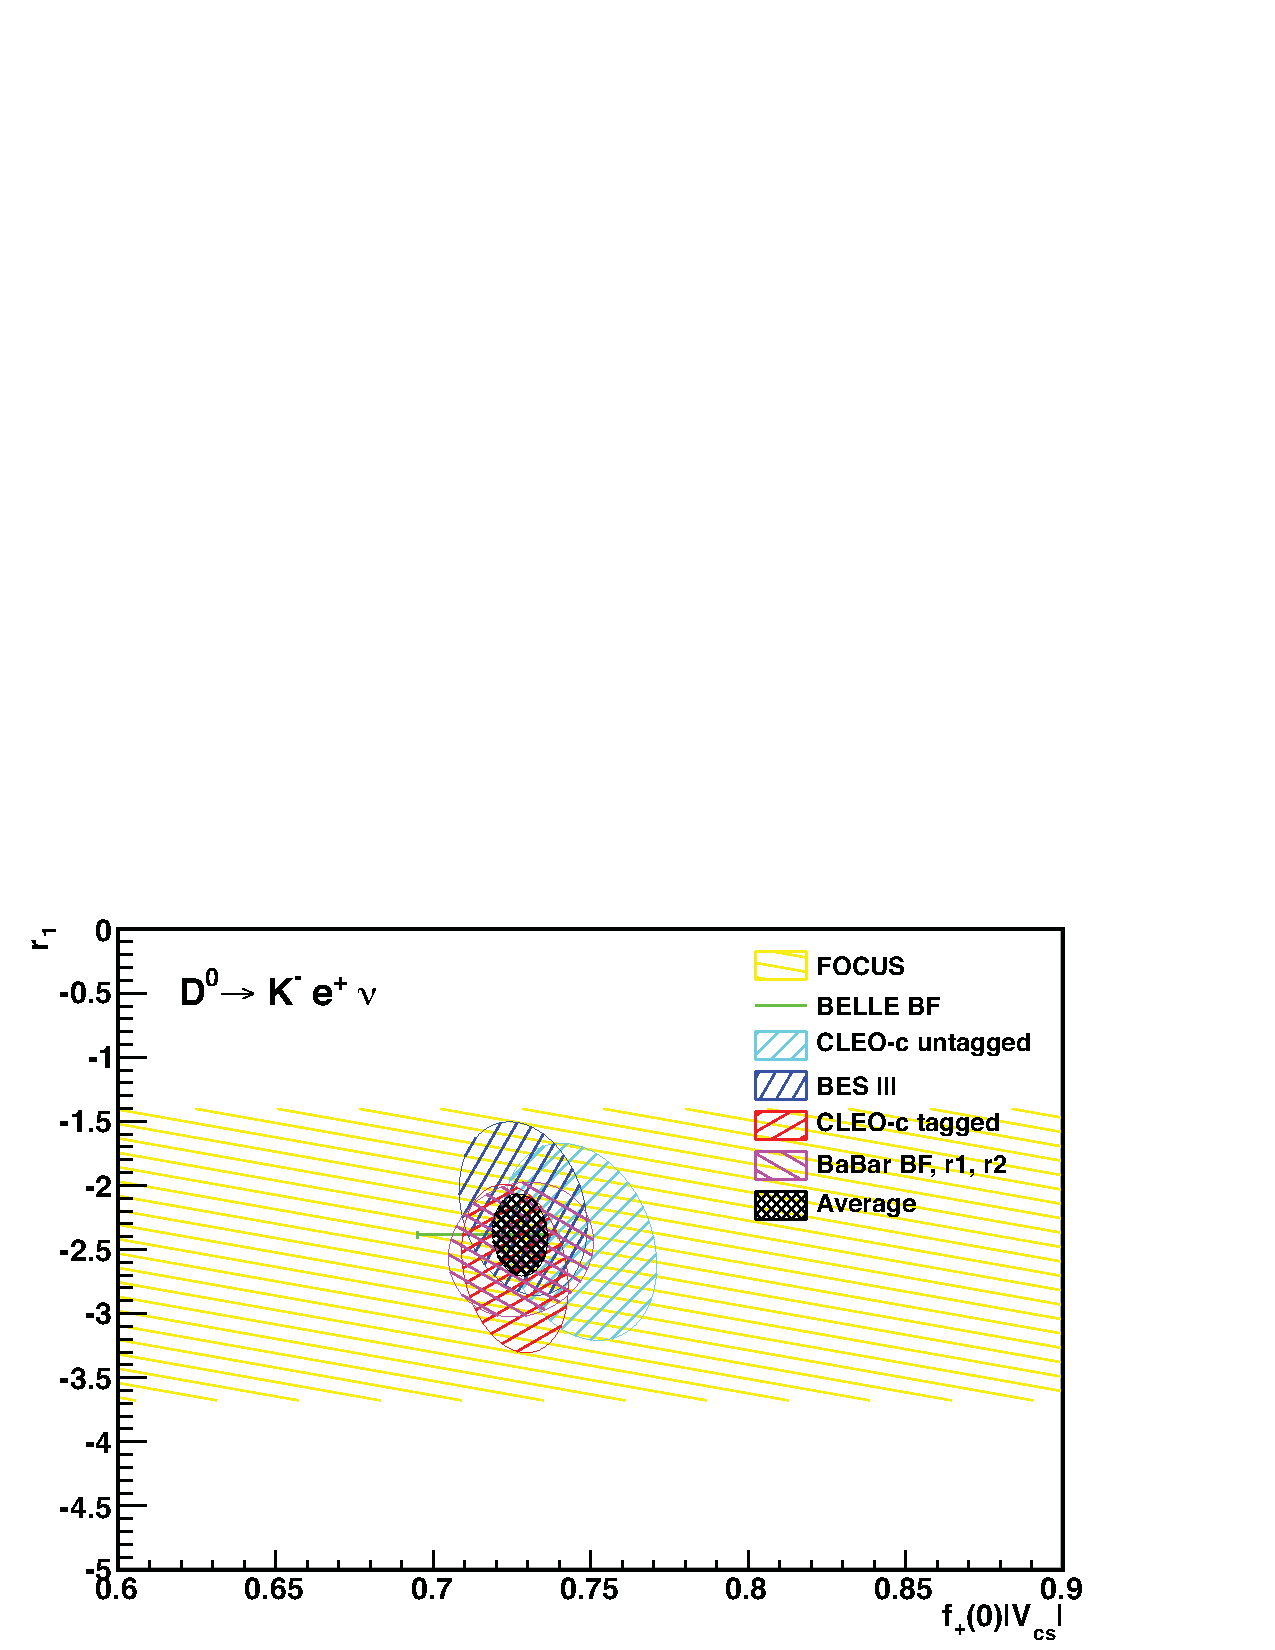
\includegraphics[bb= 0 0 521 356, width=0.48\textwidth]{figures/charm/Kenu_f0r1_ellipses.pdf}\hfill
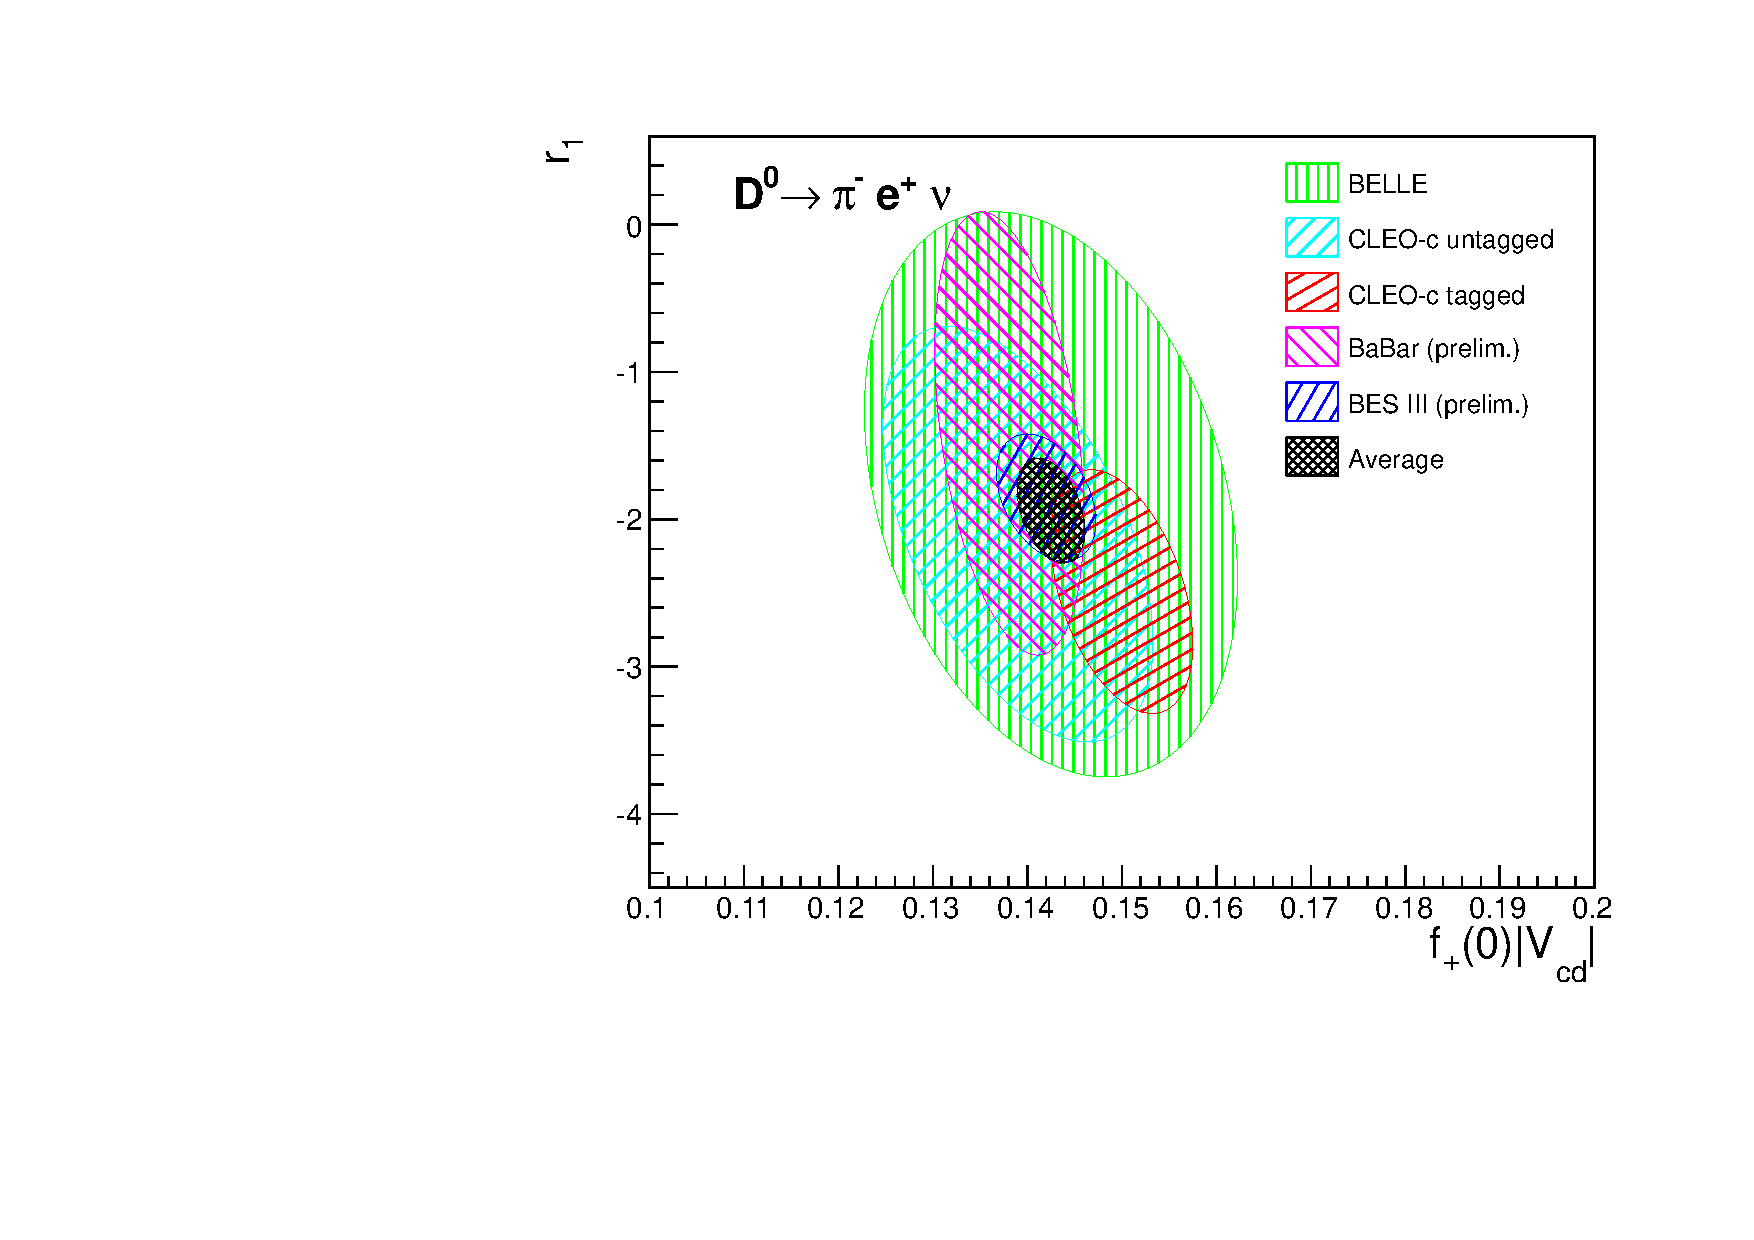
\includegraphics[width=0.48\textwidth]{figures/charm/sl_new_f0r1_pi.pdf}
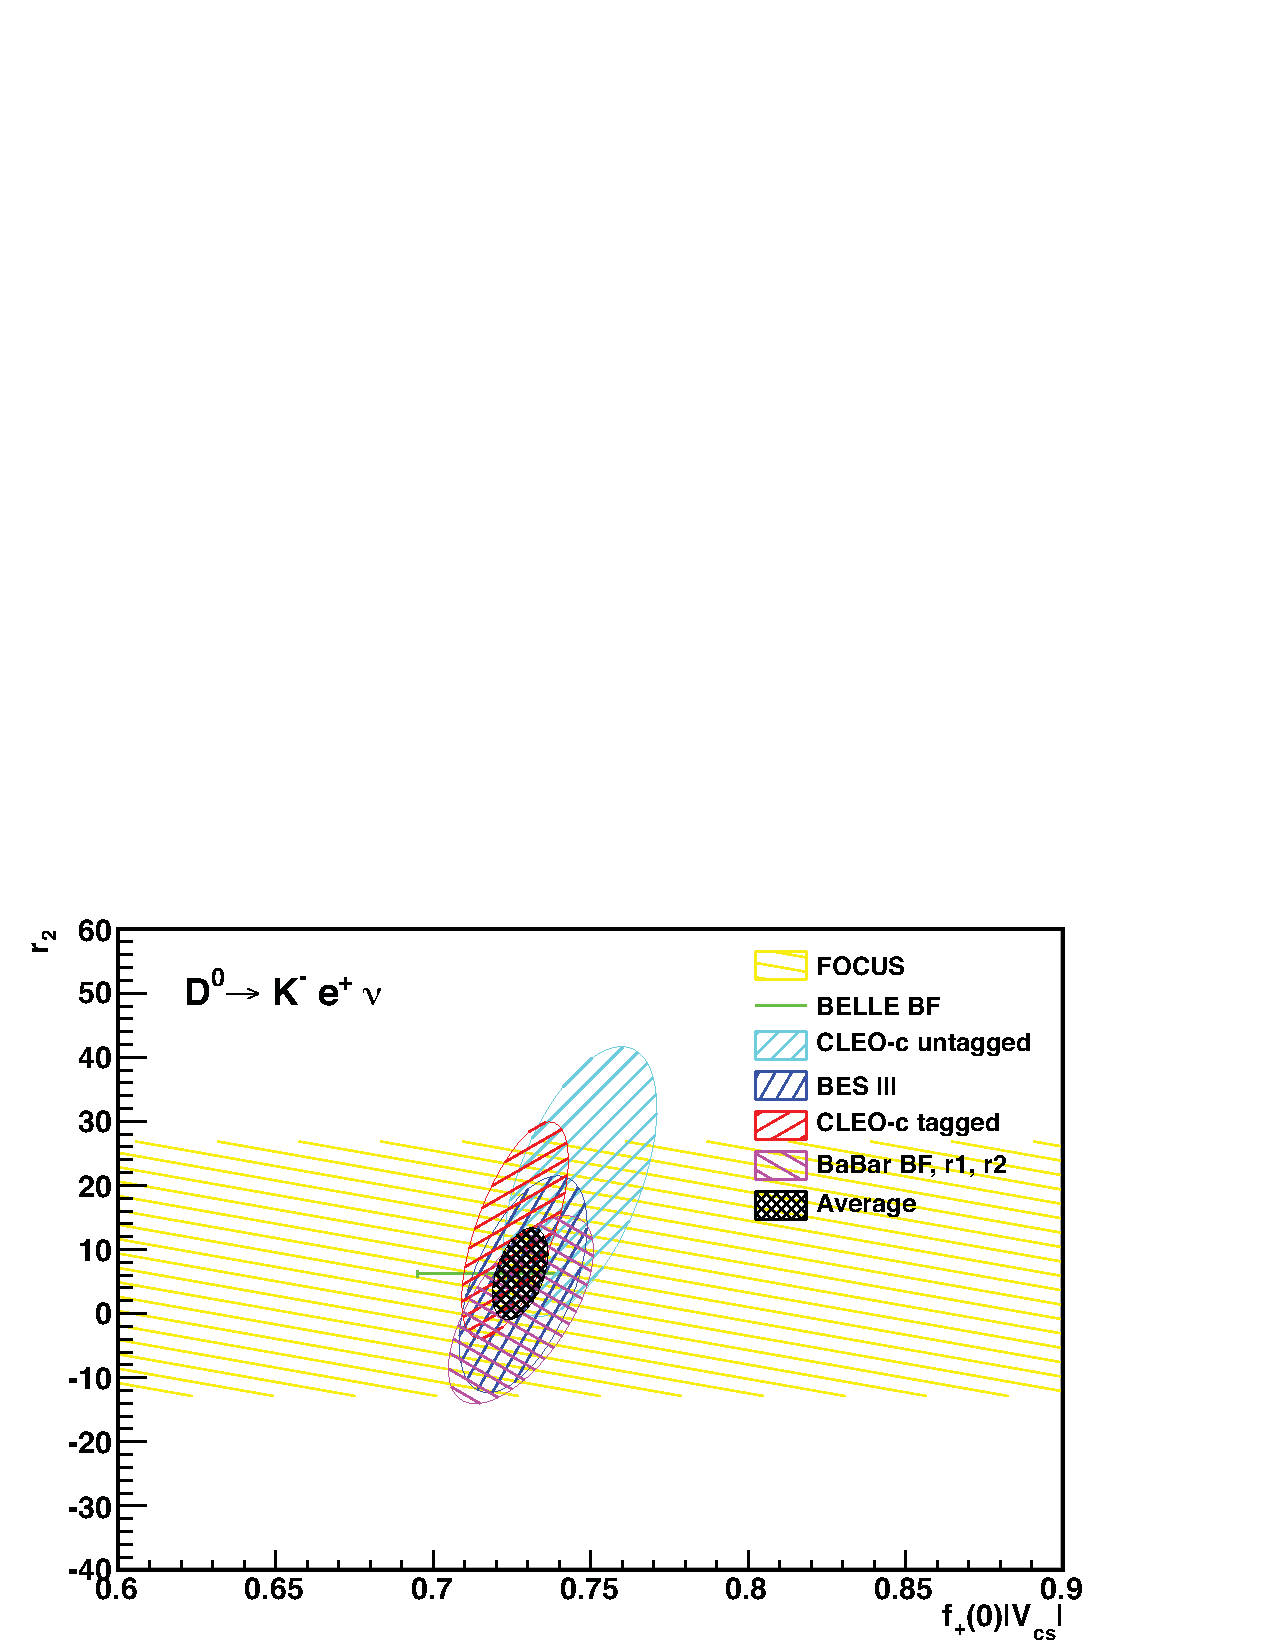
\includegraphics[bb= 0 0 521 356, width=0.48\textwidth]{figures/charm/Kenu_f0r2_ellipses.pdf}\hfill
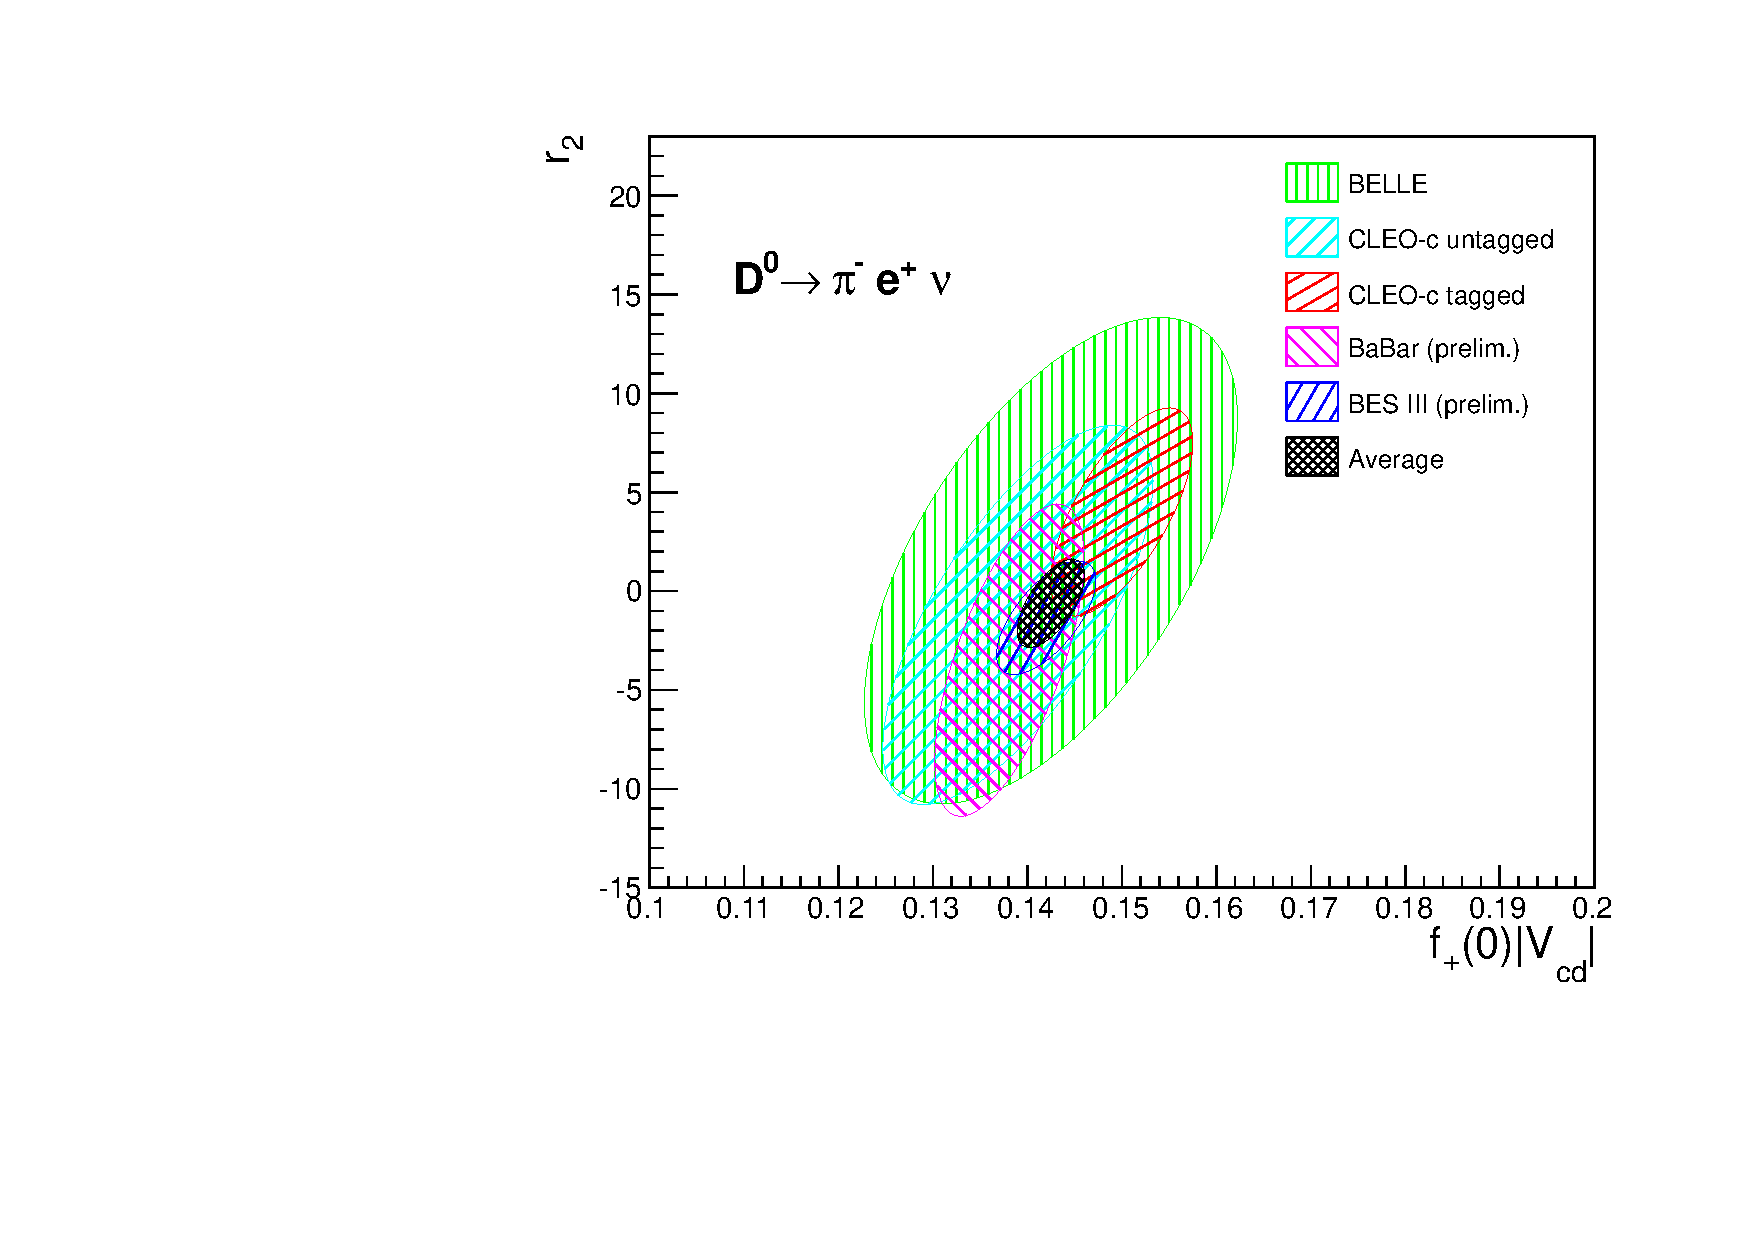
\includegraphics[width=0.48\textwidth]{figures/charm/sl_new_f0r2_pi.pdf}\hfill
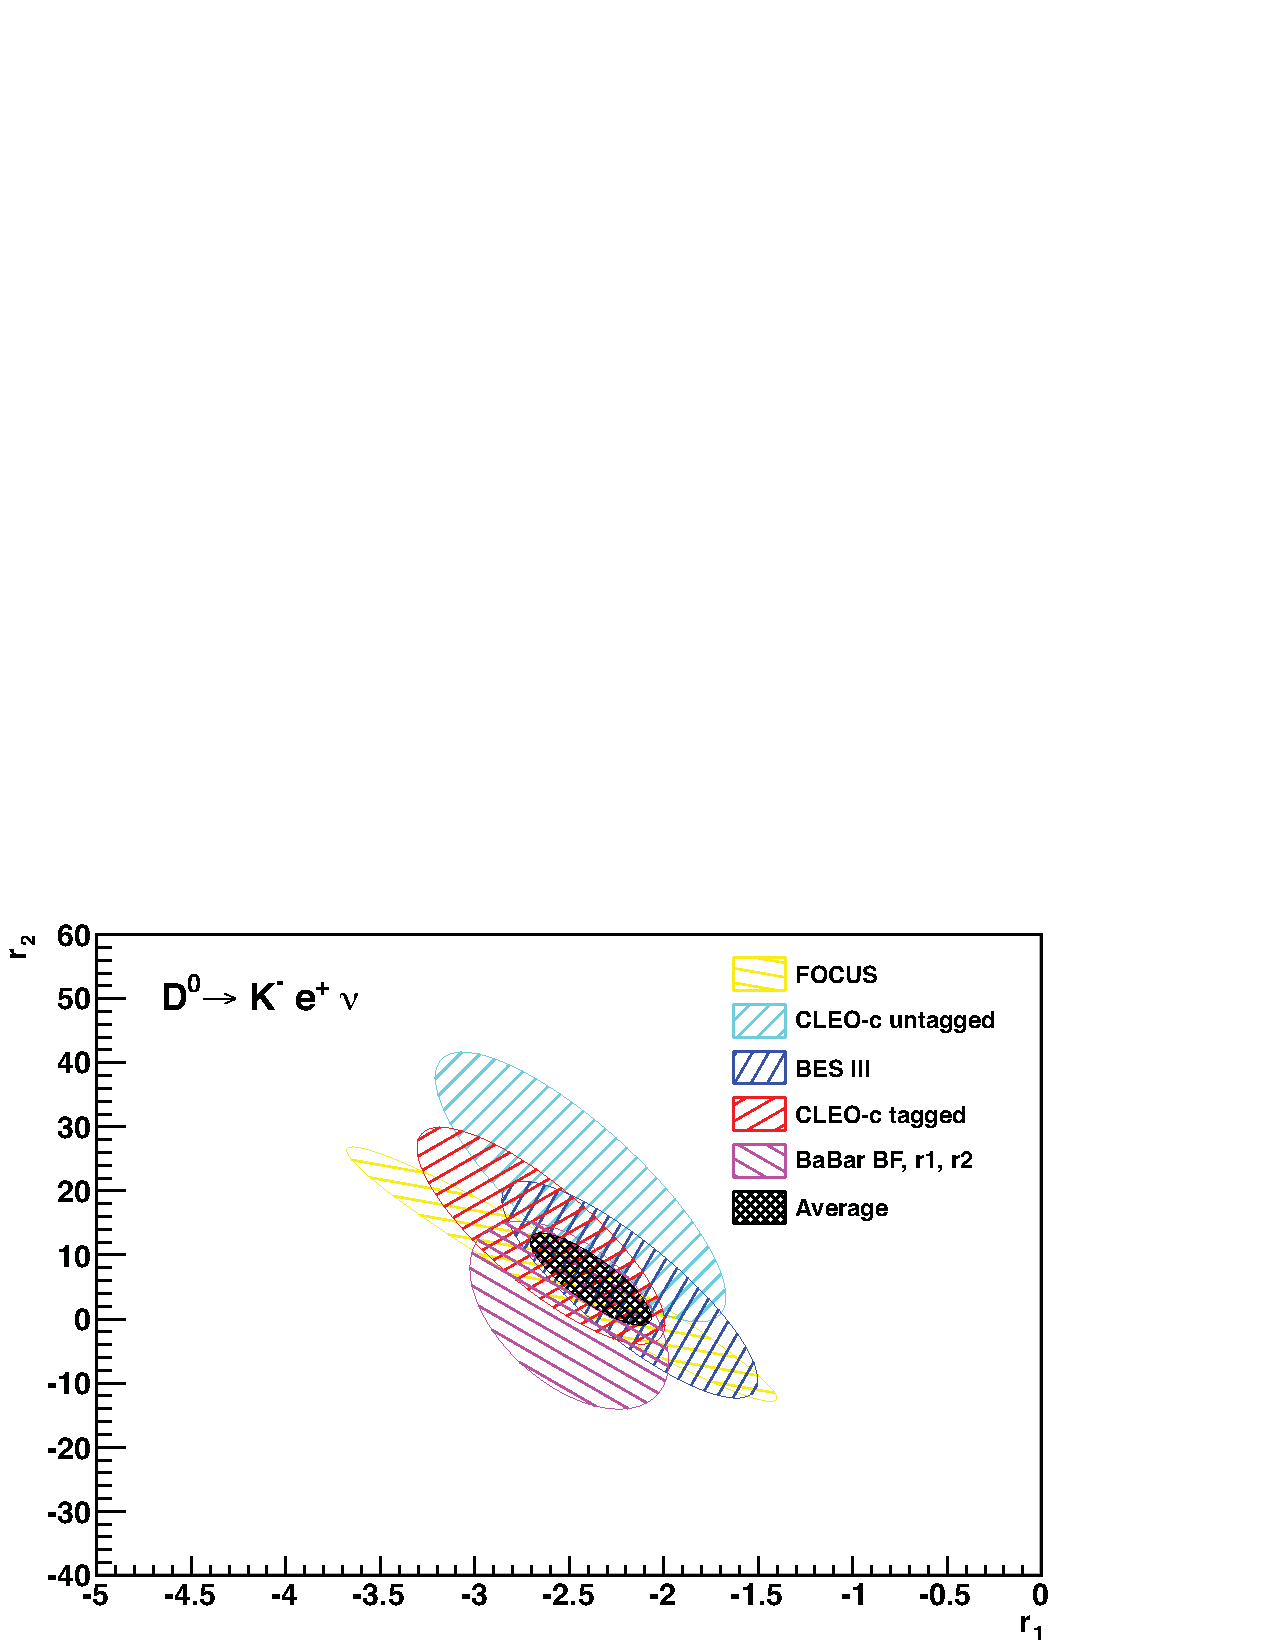
\includegraphics[bb=  0 0 520 356, width=0.48\textwidth]{figures/charm/Kenu_r1r2_ellipses.pdf}\hfill
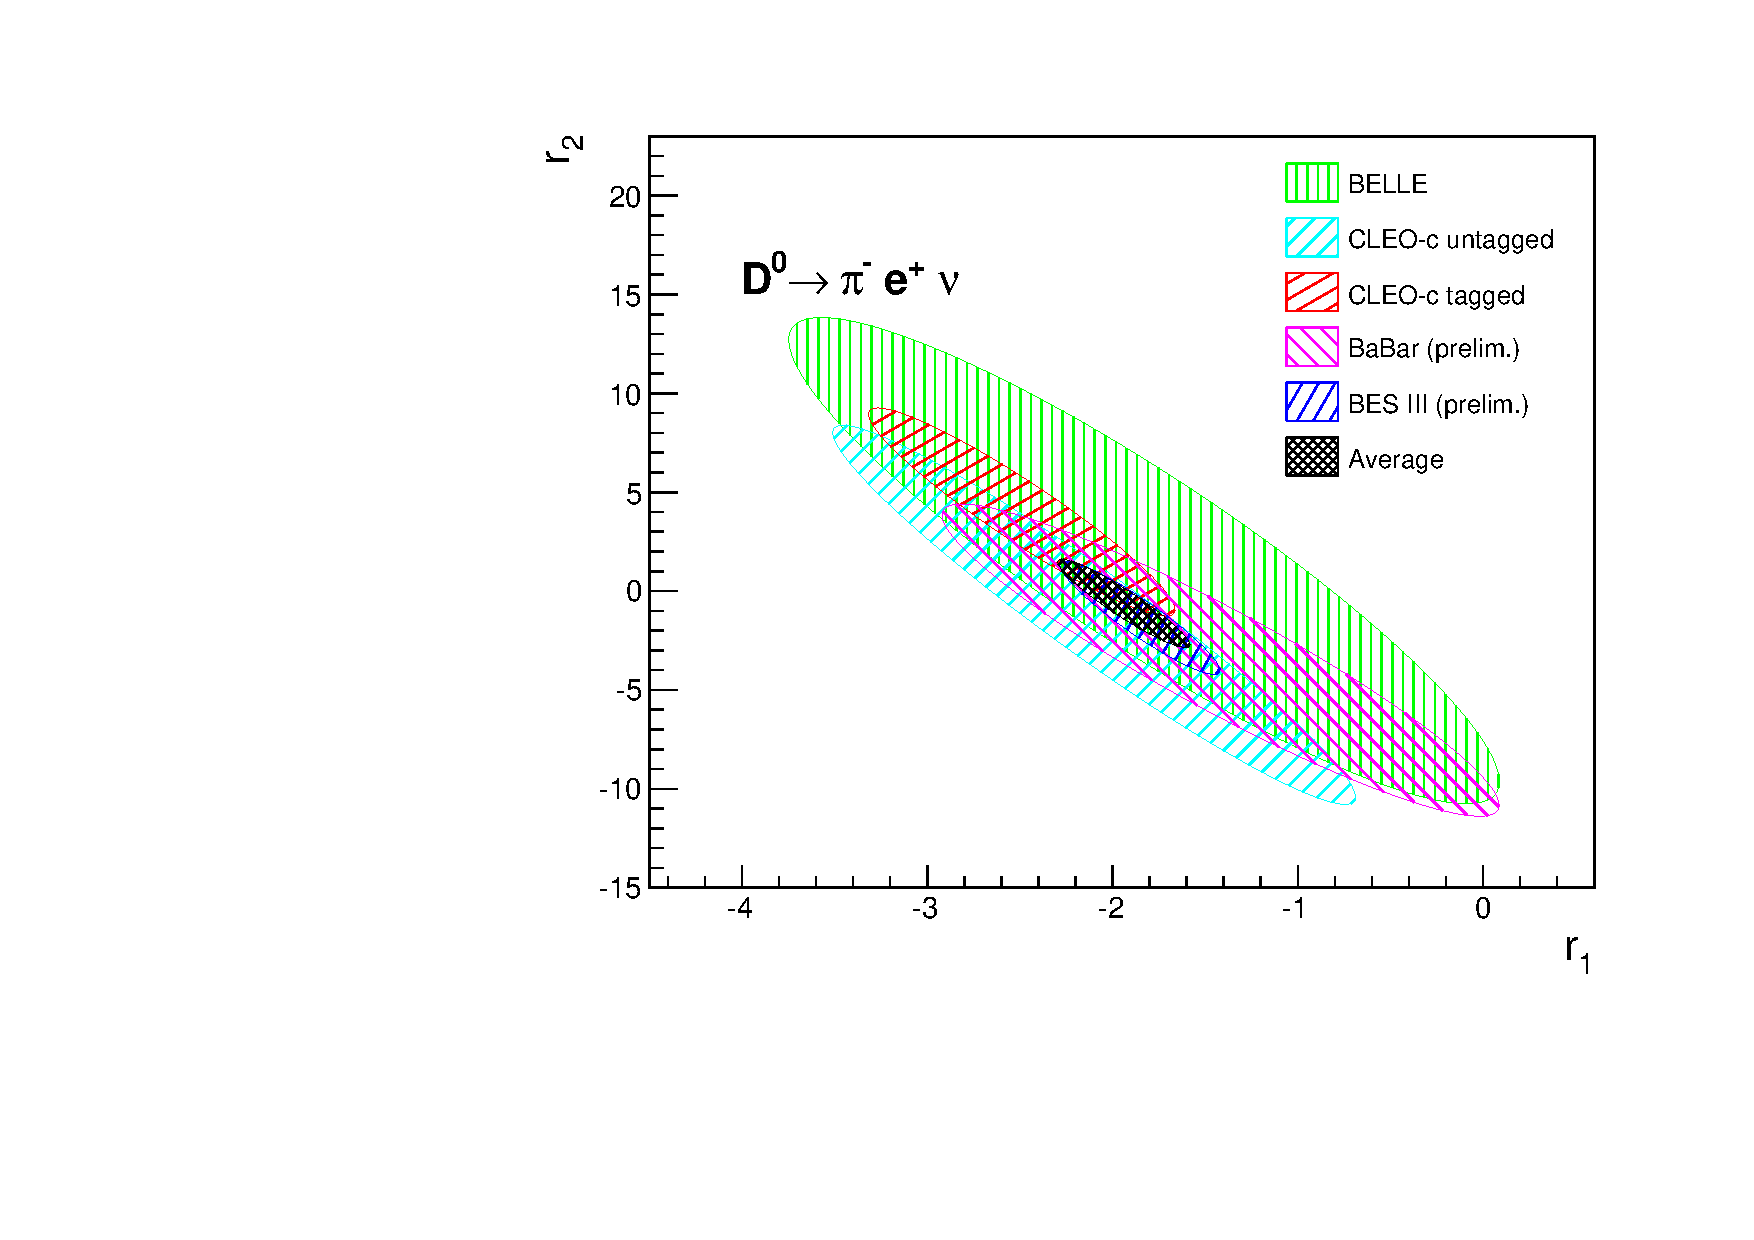
\includegraphics[width=0.48\textwidth]{figures/charm/sl_new_r1r2_pi.pdf}
\caption{The $D^0\to K^-e^+\nu$ (left) and $D^0\to \pi^-e^+\nu$ (right) 68\% C.L. error ellipses from the
average fit of the 3-parameter $z$-expansion results. 
\label{fig:fitellipse}}
\end{center}
\end{figure}

%\begin{figure}[htbp]
%  \begin{center}
%    \includegraphics[width=0.5\textwidth,angle=-90]{figures/charm/Kenu_f0r1_ellipses.ps}
%  \end{center}
%\vskip0.10in
%  \caption{Results of the combined 
%fit for $r_1$ vs $f_+(0)|V_{cs}|$. Ellipses show the 1$\sigma$ contour.    
%  \label{fig:f0r1}}
%\end{figure}

%\begin{figure}[htbp]
%  \begin{center}
%    \includegraphics[width=0.5\textwidth,angle=-90]{figures/charm/Kenu_f0r2_ellipses.ps}
%  \end{center}
%\vskip0.10in
%  \caption{Results of the combined fit for $r_2$ vs $f_+(0)|V_{cs}|$. 
%Ellipses show the 1$\sigma$ contour.
%  \label{fig:f0r2}}
%\end{figure}

%\begin{figure}[htbp]
%  \begin{center}
%    \includegraphics[width=0.5\textwidth,angle=-90]{figures/charm/Kenu_r1r2_ellipses.ps}
%  \end{center}
%\vskip0.10in
%  \caption{Results of the combined fit for $r_1$ vs $r_2$. 
%Ellipses show the 1$\sigma$ contour.
%  \label{fig:r1r2}}
%\end{figure}


\begin{table}[!htb]
\begin{center}
 \caption[]{Results for the form factor normalization
$f_+^K(0)|V_{cs}|$ and $f_+^{\pi}(0)|V_{cd}|$. Results from the
different collaborations have been corrected, if needed, using
values from PDG 2010~\cite{PDG_2010}. 
Prior to 2006, and apart from BES II, experiments
measure the ratio $(f_+^{\pi}(0)|V_{cd}| / f_+^K(0)|V_{cs}|)^2$. 
Corresponding values given in this Table for $f_+^{\pi}(0)|V_{cd}|$
are obtained by assuming that $f_+^K(0)|V_{cs}|=0.714\pm 0.009$.
Results of the combined fit include measurements from 2006 and later. 
%for experiments measuring $f_+(0)|V_{cq}|$, $r_1$ and $r_2$. 
%In the case of the $D \to \pi \ell \nu$ decay channel, Belle results refitted 
%with the z-expansion, and the \babar and BES III preliminary results are included.
Results of CLEO (2008) (untagged) shown in this table only refer to the $D^0$ channel.
%are not included in this average because they are 
%superseeded by those of CLEO (2009).
%Results from LQCD are given in the last line \cite{Na:2010uf} \cite{Na:2011mc}.}
%Published results are multiplied by 
%$|V_{cs}|=0.9729\pm0.003$ and $|V_{cd}| = 0.2253 \pm 0.009$ from unitarity.
%Results quoted for LQCD are obtained by multiplying the values
%computed for $f_+^K(0)$ and $f_+^{\pi}(0)$ from lattice by
%$|V_{cs}|=0.9729$ and $|V_{cd}|=0.2253$ respectively. These
%values of $|V_{cs(d)}|$ correspond to present estimates assuming
%the unitarity of the CKM matrix.
Values entering in the combination explained before are marked with a $\ast$. 
In the combination only the result for the $D \to \pi \ell \nu_\ell $ channel is obtained 
with the total BES III statistics \cite{BESIII-new}, while the $D \to K \ell \nu_\ell $ 
channel includes results with partial statistics \cite{BESIII}.
 \label{norma}}
\resizebox{\textwidth}{!}{
\begin{tabular}{c c c c}
\vspace*{-10pt} & \\
\hline
Experiment & Ref. & $f_+^K(0)|V_{cs}|$ & $f_+^{\pi}(0)|V_{cd}|$ \\
\hline\hline 
E691 (1989)&\cite{Anjos:1988ue} & $0.69 \pm 0.05\pm 0.05 $ &  \\
CLEO (1991) &\cite{Crawford:1991zd} & $$ &  \\
CLEOII (1993) &\cite{Bean:1993zv}  & $0.76 \pm 0.01 \pm 0.04$ &  \\
CLEOII (1995) &\cite{Butler:1995ca}  & &$0.163 \pm 0.031 \pm 0.011$  \\
E687 (1995) &\cite{Frabetti:1995xq} & $0.69\pm 0.03\pm 0.03 $ &  \\
E687 (1996) &\cite{Frabetti:1996jj} &  &$0.160 \pm 0.018 \pm 0.004$  \\
BESII (2004) &\cite{Ablikim:2004ej} &$0.78 \pm 0.04 \pm 0.03$ & $0.164 \pm 0.032 \pm0.014$   \\
CLEOIII (2005) &\cite{Huang:2004fra} & &$0.139^{+0.011~+0.009}_{-0.013~-0.006}$ \\
FOCUS (2005)  & \cite{Link:2004dh} & &$0.137 \pm 0.008 \pm 0.008$ \\
\hline
Belle (2006) $\ast$ & \cite{Widhalm:2006wz}& $0.692 \pm 0.007 \pm 0.022$ & $0.140\pm 0.004\pm0.007$ \\ 
\babar (2007) $\ast$,(preliminary 2014) $\ast$ & \cite{Aubert:2007wg,babar-new} & $0.720 \pm 0.007\pm 0.007$ & $0.137 \pm 0.004\pm 0.002$  \\
CLEO-c (2008)(untagged) $\ast$ &\cite{Dobbs:2007aa} & $0.747 \pm 0.009\pm 0.009$ & $0.139 \pm 0.007\pm 0.003$ \\
CLEO-c (2009) (tagged) $\ast$ &\cite{Besson:2009uv} & $0.719 \pm 0.006\pm 0.005$ & $0.150 \pm 0.004\pm 0.001$ \\
%BESIII (2012)(prel.) $\ast$ &\cite{BESIII} & $0.729 \pm 0.008\pm 0.007$ & $0.144 \pm 0.005\pm 0.002$ \\
BESIII (2012, 2014) (preliminary) $\ast$ &\cite{BESIII-new} & $0.720 \pm 0.004\pm 0.004$ & $0.142 \pm 0.002\pm 0.001$ \\ 
\hline\hline
% Combined fit                & \omit      & $ 0.728 \pm 0.005 $               &       $ 0.146 \pm 0.003$   \\
 Combined fit (preliminary)                & \omit      & $ 0.728 \pm 0.005 $               &       $ 0.1425 \pm 0.0019$   \\
\hline
\hline
%HPQCD & \cite{Na:2011mc}\cite{Na:2010uf}             & $0.727\pm0.018$         & $0.150 \pm 0.007$      \\
%\vspace*{-10pt} & \\
%\hline
\end{tabular}
}
\end{center}
\end{table}

\vspace{0.5cm}
Results of fits of the three-pole model~\cite{Becirevic:2014kaa} to  $D \to \pi \ell \nu_\ell $ data from \babar~\cite{babar-new}, Belle\cite{Widhalm:2006wz}, BES III\cite{BESIII-new} and 
CLEOc~\cite{Besson:2009uv,Dobbs:2007aa} are shown in Table~\ref{3Pole_pi}. 
The fitted parameters are the first two residues $\gamma_{0}=\underset{ q^2=m_{D^{\ast}}^2} {\rm Res} f_+(q^2) $ 
and $\gamma_{1}=\underset{q^2=m_{D^{\ast '}}^2}{\rm Res} f_+(q^2)$ (which are constrained using present measurements 
of masses and widths of the $D^\ast$ and $D^{\ast '}$ mesons, and lattice computations of decay constants, following Ref.~\cite{Becirevic:2014kaa}), 
and an effective mass, $m_{D^{\ast ''}_{eff}}$, accounting for higher mass hadronic contributions.
The $V_{cd}$ value enters in the fit and is constrained assuming unitarity of the CKM matrix.
The $\chi^2/d.o.f$ of the combined fit is $57.5/57$. The result of the effective mass $m_{D^{\ast ''}_{eff}}$ is larger than the mass of the 
second radially excited state with $J^P = 1^{-}$ ($\sim 3.11$~GeV), indicating that more contributions are needed to explain the form factor. 
Comparison of the combined fit with the individual data is shown in Figure@\ref{plot3}.

\begin{figure}[p]
\begin{center}
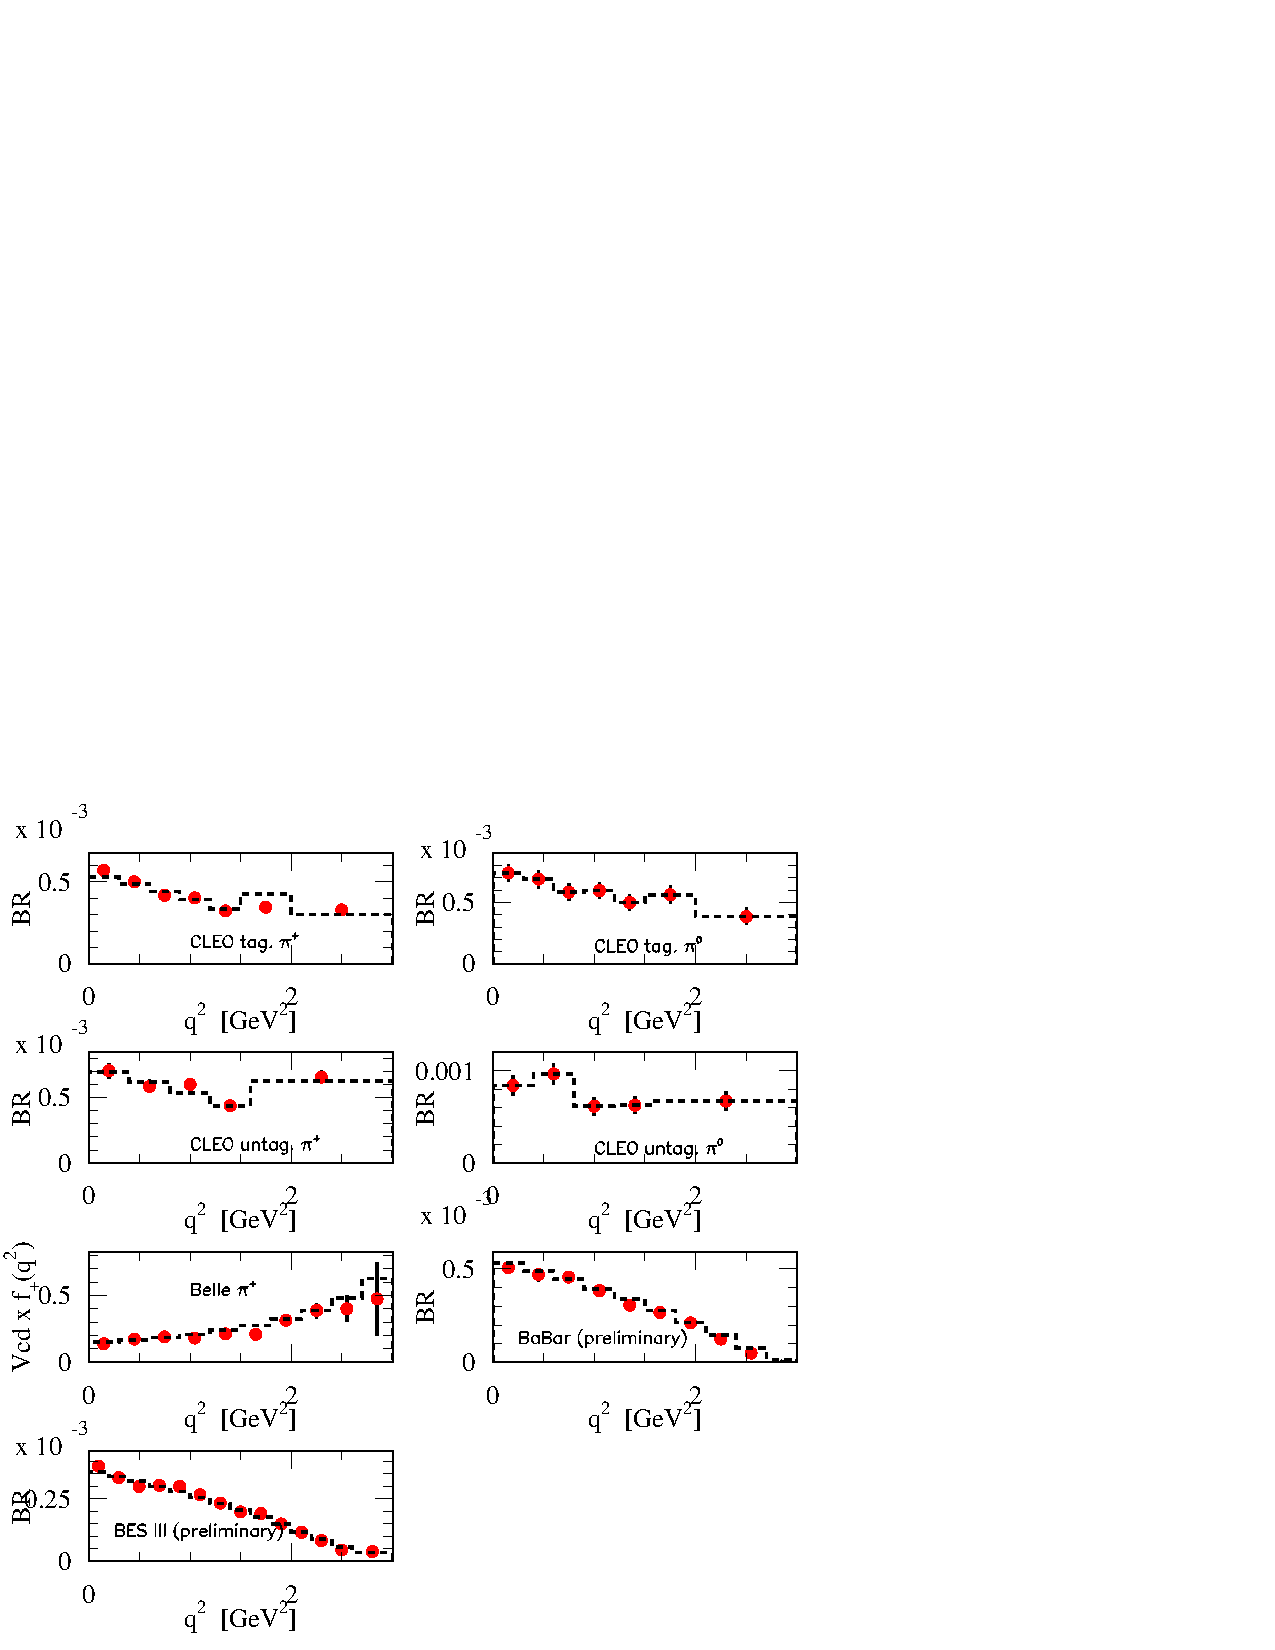
\includegraphics[bb = 0 0 425 425, width=1\textwidth]{figures/charm/sl_plot3.pdf}
\caption{Result of the three-pole model fit \cite{Becirevic:2014kaa} to \babar~\cite{babar-new}, Belle\cite{Widhalm:2006wz}, 
BES III\cite{BESIII-new} and CLEOc~\cite{Besson:2009uv,Dobbs:2007aa} $D \to \pi \ell \nu_\ell $ data. Red points are the 
measured data in $q^2$ bins and the black line correspond to the result of the combined fit.
\label{plot3}
}
\end{center}
\end{figure}

%For the Belle measurement published values of $f^{D\pi}_{+} (q^2) \times |V_{cd}|$ have been modifyied by subtracting the $V_{cd}$ 
%uncertainty from the total systematic error.

\begin{table}[htbp]
\caption{Results of the three-pole model to \babar (preliminary), Belle, BES III (preliminary) and CLEOc (tagged and untagged) data. 
Fitted parameters are the first two residues 
$\gamma_0$  and $\gamma_{1}$, which are constrained using present measurements 
of masses and widths of the $D^\ast$ and $D^{\ast '}$ mesons, and lattice computations of decay constants, and the effective mass,  
$m_{D^{\ast ''}_{eff}}$, 
accounting for higher mass hadronic contributions. 
\label{3Pole_pi}}
\begin{center}
\begin{tabular}{cc}
\hline 
Parameter & Combined result ($D \to \pi \ell \nu_\ell $) \\ 
\hline 
\vspace*{-10pt} & \\
\hline
$\gamma_0$  & 3.878 $\pm$ 0.090  GeV$^2$ \\
$\gamma_1$  & -1.18 $\pm$ 0.30  GeV$^2$  \\
$m_{D^{\ast ''}_{eff}}$  & 4.17 $\pm$ 0.41 GeV \\
%$V_{cd}$ & 0.22506 $\pm$ 0.00087\\
\hline
\vspace*{-10pt} & \\
\hline
\end{tabular}
\end{center}
\end{table}

\subsubsection{$D\ra V\overline \ell \nu_\ell$ decays}

When the final state hadron is a vector meson, the decay can proceed through
both vector and axial vector currents, and four form factors are needed.
The hadronic current is $H^{}_\mu = V^{}_\mu + A^{}_\mu$, 
where~\cite{Gilman:1989uy} 
\begin{eqnarray}
V_\mu & = & \left< V(p,\varepsilon) | \bar{q}\gamma^\mu c | D(p') \right> \ =\  
\frac{2V(q^2)}{m_D+m_V} 
\varepsilon_{\mu\nu\rho\sigma}\varepsilon^{*\nu}p^{\prime\rho}p^\sigma \\
 & & \nonumber\\
A_\mu & = & \left< V(p,\varepsilon) | -\bar{q}\gamma^\mu\gamma^5 c | D(p') \right> 
 \ =\  -i\,(m_D+m_V)A_1(q^2)\varepsilon^*_\mu \nonumber \\
 & & \hskip2.10in 
  +\ i \frac{A_2(q^2)}{m_D+m_V}(\varepsilon^*\cdot q)(p' + p)_\mu \nonumber \\
 & & \hskip2.30in 
+\ i\,\frac{2m_V}{q^2}\left(A_3(q^2)-A_0(q^2)\right)[\varepsilon^*\cdot (p' + p)] q_\mu\,.
\end{eqnarray}
In this expression, $m_V$ is the daughter meson mass and
\begin{eqnarray}A_3(q^2) & = & \frac{m_D + m_V}{2m_V}A_1(q^2)\ -\ \frac{m_D - m_V}{2m_V}A_2(q^2)\,.
\end{eqnarray}
Kinematics require that $A_3(0) = A_0(0)$.
The differential partial width is
%integrated over various angular distributions is
\begin{eqnarray}
\frac{d\Gamma(D \to V \overline \ell \nu_\ell)}{dq^2\, d\cos\theta_\ell} & = & 
  \frac{G_F^2\,|V_{cq}|^2}{128\pi^3m_D^2}\,p^*\,q^2 \times \nonumber \\
 & &  
\left[\frac{(1-\cos\theta_\ell)^2}{2}|H_-|^2\ +\  
\frac{(1+\cos\theta_\ell)^2}{2}|H_+|^2\ +\ \sin^2\theta_\ell|H_0|^2\right]\,,
\end{eqnarray}
where $H^{}_\pm$ and $H^{}_0$ are helicity amplitudes given by
\begin{eqnarray}
H_\pm & = & \frac{1}{m_D + m_V}\left[(m_D+m_V)^2A_1(q^2)\ \mp\ 
      2m^{}_D\,p^* V(q^2)\right] \\
 & & \nonumber \\
H_0 & = & \frac{1}{|q|}\frac{m_D^2}{2m_V(m_D + m_V)}\ \times\ \nonumber \\
 & & \hskip0.01in \left[
    \left(1- \frac{m_V^2 - q^2}{m_D^2}\right)(m_D + m_V)^2 A_1(q^2) 
    \ -\ 4{p^*}^2 A_2(q^2) \right]\,.
\label{HelDef}
\end{eqnarray}
$p^*$ is the magnitude of the three-momentum of the $K \pi$ system, measured in the $D$ rest frame.
The left-handed nature of the quark current manifests itself as
$|H_-|>|H_+|$. The differential decay rate for $D\ra V\ell\nu$ 
followed by the vector meson decaying into two pseudoscalars is

\begin{eqnarray}
\frac{d\Gamma(D\ra V\ell\nu, V\ra P_1P_2)}{dq^2 d\cos\theta_V d\cos\theta_\ell d\chi} 
 &  = & \frac{3G_F^2}{2048\pi^4}
       |V_{cq}|^2 \frac{p^*(q^2)q^2}{m_D^2} {\cal B}(V\to P_1P_2)\ \times \nonumber \\ 
 & & \hskip0.10in \big\{ (1 + \cos\theta_\ell)^2 \sin^2\theta_V |H_+(q^2)|^2 \nonumber \\
 & & \hskip0.20in +\ (1 - \cos\theta_\ell)^2 \sin^2\theta_V |H_-(q^2)|^2 \nonumber \\
 & & \hskip0.30in +\ 4\sin^2\theta_\ell\cos^2\theta_V|H_0(q^2)|^2 \nonumber \\
 & & \hskip0.40in +\ 4\sin\theta_\ell (1 + \cos\theta_\ell) 
             \sin\theta_V \cos\theta_V \cos\chi H_+(q^2) H_0(q^2) \nonumber \\
 & & \hskip0.50in -\ 4\sin\theta_\ell (1 - \cos\theta_\ell) 
          \sin\theta_V \cos\theta_V \cos\chi H_-(q^2) H_0(q^2) \nonumber \\
 & & \hskip0.60in -\ 2\sin^2\theta_\ell \sin^2\theta_V 
                \cos 2\chi H_+(q^2) H_-(q^2) \big\}\,,
\label{eq:dGammaVector}
\end{eqnarray}
where the angles $\theta^{}_\ell$, $\theta^{}_V$, and $\chi$ are defined
in Fig.~\ref{DecayAngles}. 

\begin{figure}[htbp]
  \begin{center}
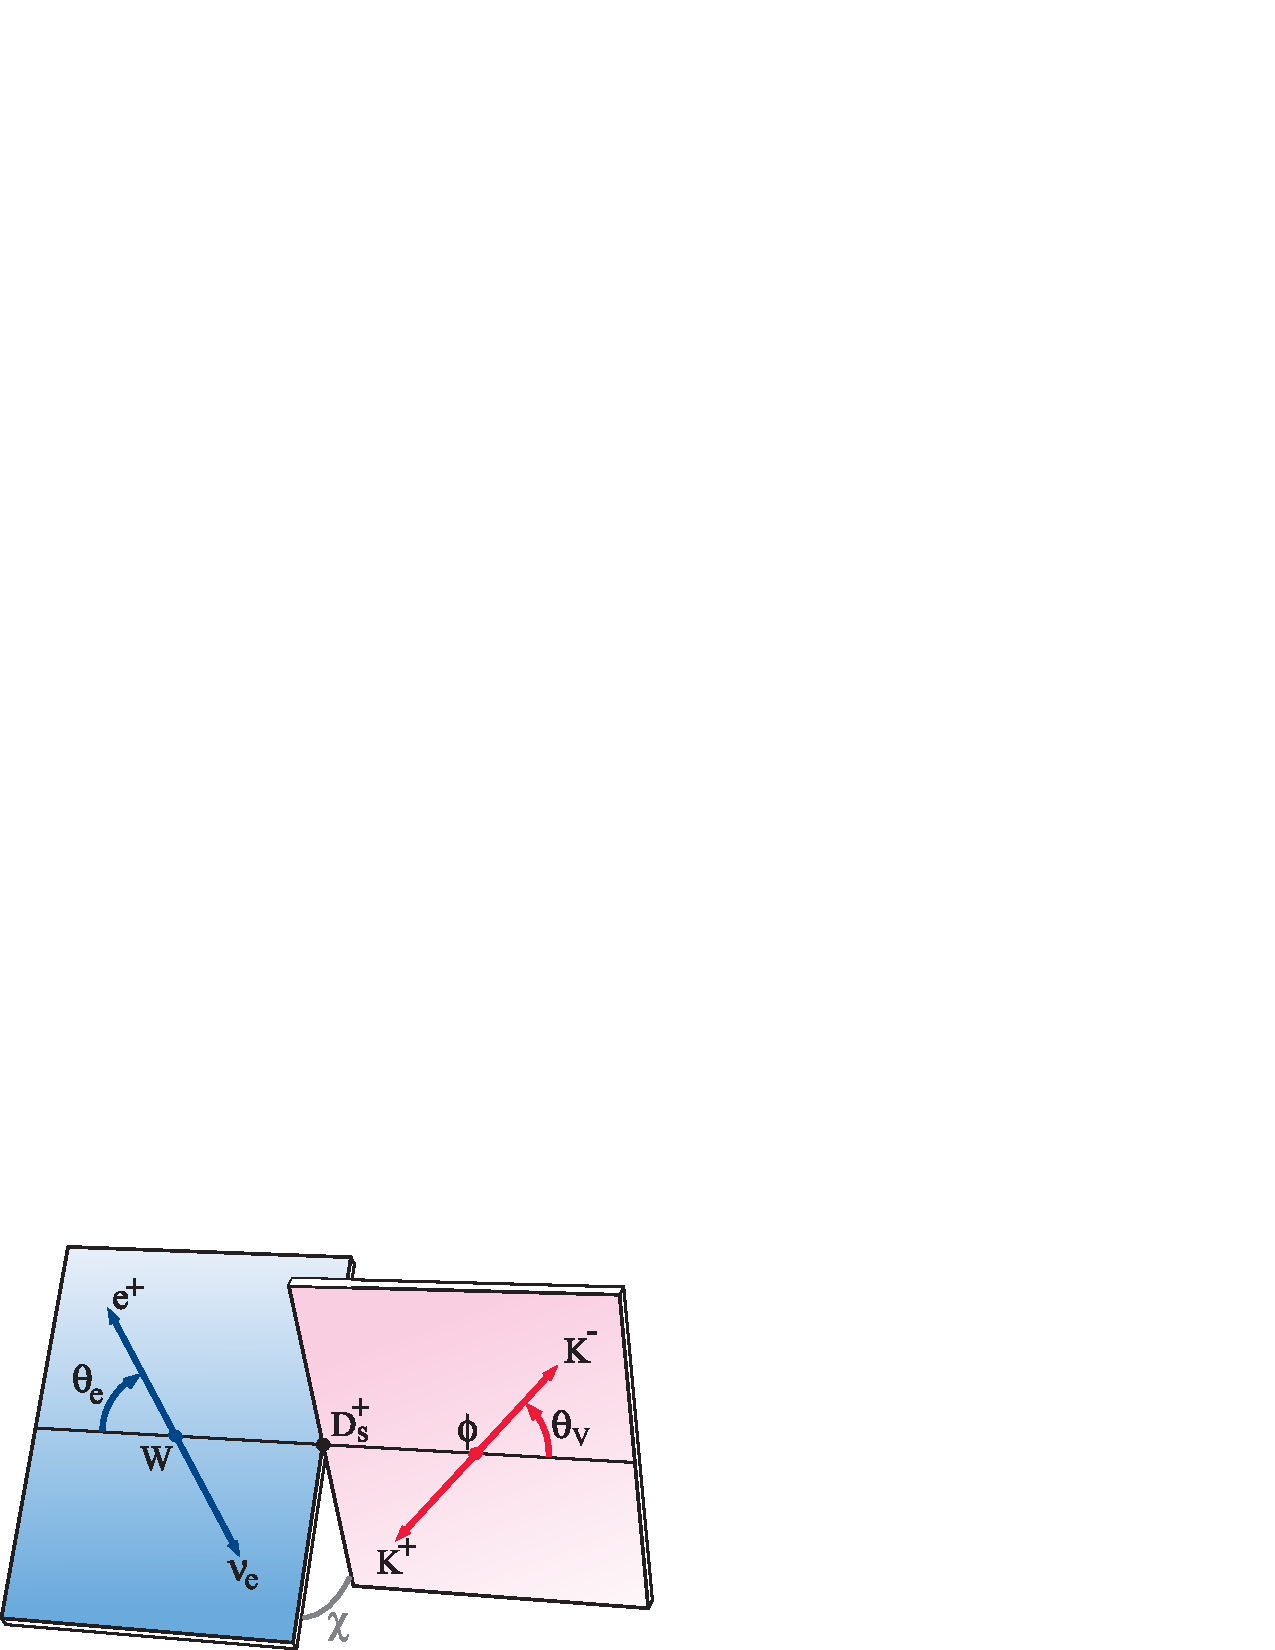
\includegraphics[width=2.5in, bb=0 0 320 200]{figures/charm/sl_Widhalm07_3.pdf}
%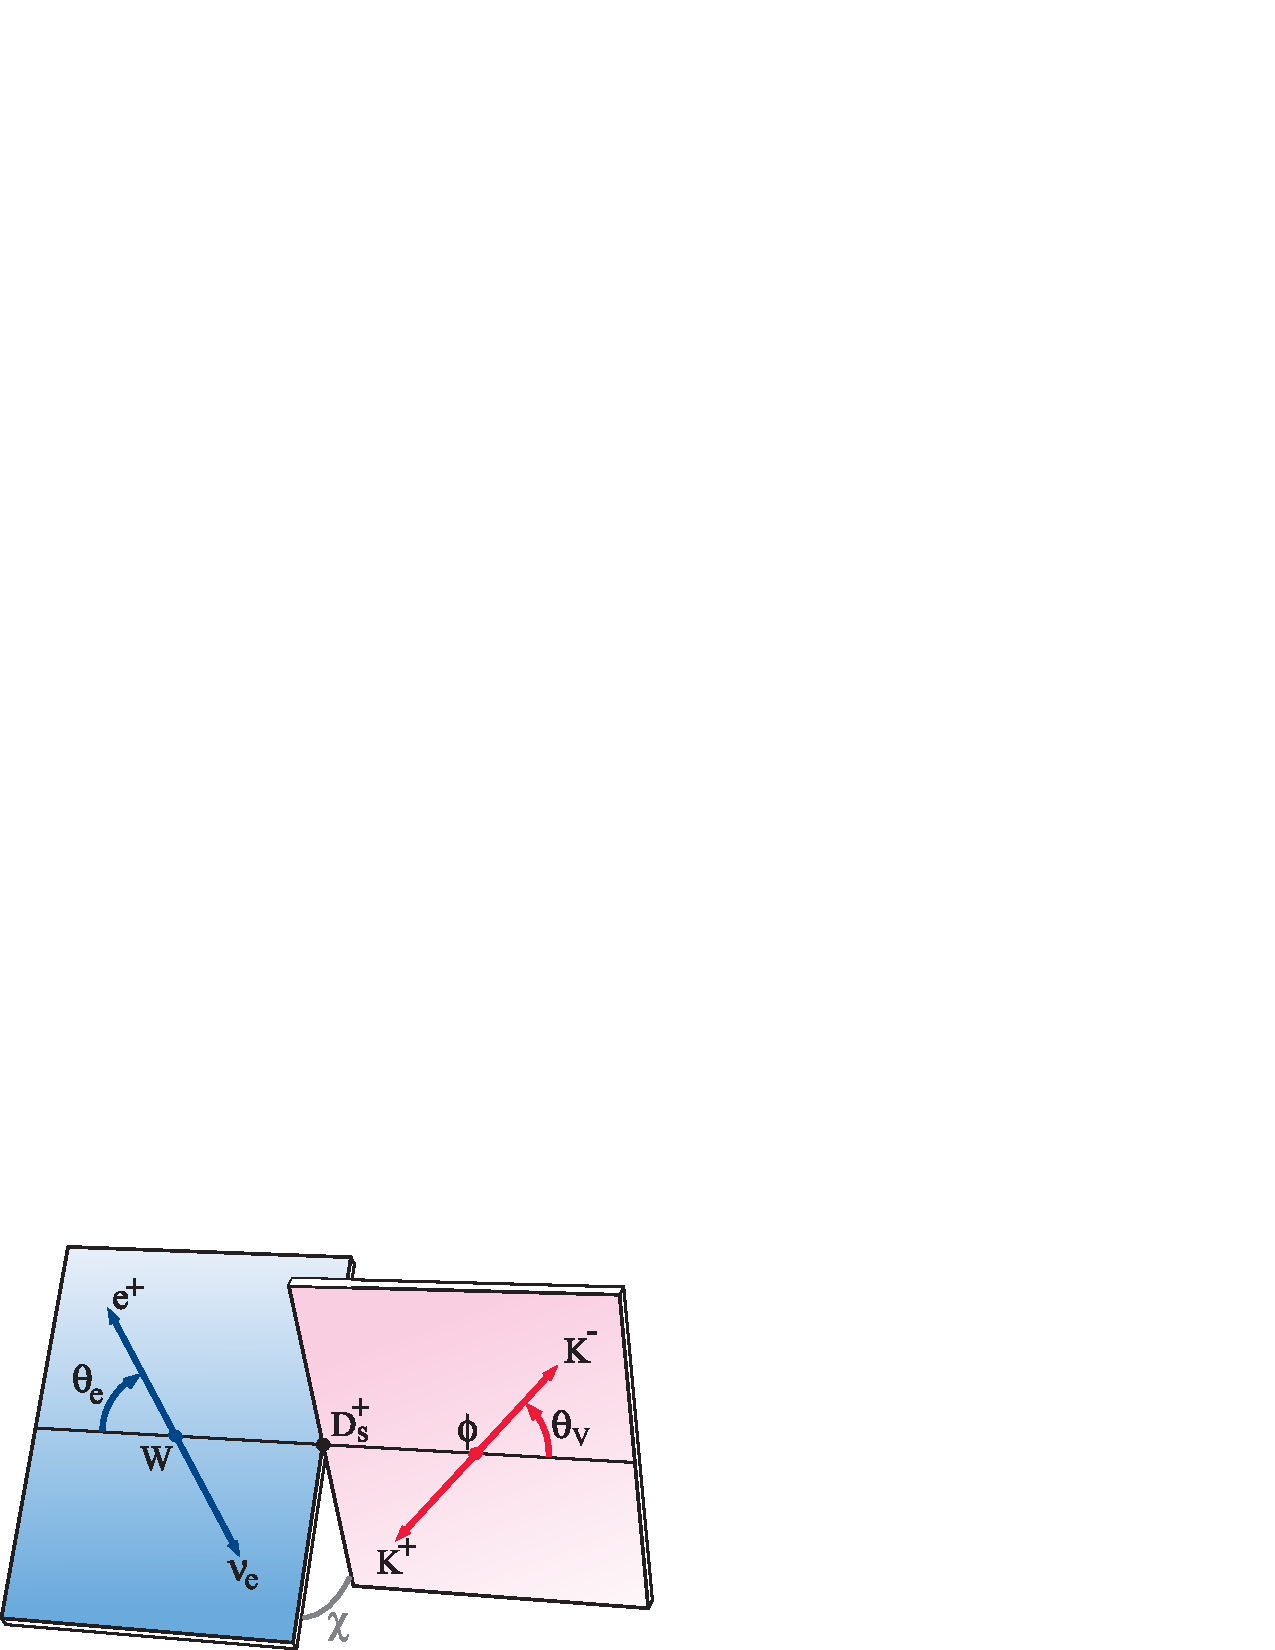
\includegraphics[width=6.50in]{figures/charm/sl_Widhalm07_3.pdf}
  \end{center}
  \caption{
    Decay angles $\theta_V$, $\theta_\ell$ 
    and $\chi$. Note that the angle $\chi$ between the decay
    planes is defined in the $D$-meson reference frame, whereas
    the angles $\theta^{}_V$ and $\theta^{}_\ell$ are defined
    in the $V$ meson and $W$ reference frames, respectively.}
  \label{DecayAngles}
\end{figure}

%Assuming that the simple pole form of Eq.~(\ref{SimplePole}) describes 
%the $q^2$-dependence of the form factors, the %four-dimensional 
%distribution of Eq.~(\ref{eq:dGammaVector}) will depend only on the parameters
Ratios between the values of the hadronic form factors expressed at $q^2=0$ are usually introduced:
\begin{eqnarray}
r_V \equiv V(0) / A_1(0), & &  r_2 \equiv A_2(0) / A_1(0) \label{rVr2_eq}\,.
\end{eqnarray}
Table \ref{Table1} lists measurements of $r_V$ and $r_2$ from several
experiments. Most of measurements assume that the $q^2$ dependence of hadronic form factors 
is given by the simple pole ansatz.
%The average results from $D^+\ra\overline{K}^{*0}\ell^+\nu$
%decays are also given. 
The measurements are plotted in
Fig.~\ref{fig:r2rv} which shows that they are all consistent.

\begin{table}[htbp]
\caption{Results for $r_V$ and $r_2$ from various experiments.
\label{Table1}}
\begin{center}
\begin{tabular}{cccc}
\hline
\vspace*{-10pt} & \\
Experiment & Ref. & $r_V$ & $r_2$ \\
\vspace*{-10pt} & \\
\hline
\vspace*{-10pt} & \\
$D^+\to \overline{K}^{*0}l^+\nu$ & \omit & \omit & \omit         \\
E691         & \cite{Anjos:1990pn}     & 2.0$\pm$  0.6$\pm$  0.3  & 0.0$\pm$  0.5$\pm$  0.2    \\
E653         & \cite{Kodama:1992tn}     & 2.00$\pm$ 0.33$\pm$ 0.16 & 0.82$\pm$ 0.22$\pm$ 0.11   \\
E687         & \cite{Frabetti:1993jq}     & 1.74$\pm$ 0.27$\pm$ 0.28 & 0.78$\pm$ 0.18$\pm$ 0.11   \\
E791 (e)     & \cite{Aitala:1997cm}    & 1.90$\pm$ 0.11$\pm$ 0.09 & 0.71$\pm$ 0.08$\pm$ 0.09   \\
E791 ($\mu$) & \cite{Aitala:1998ey}    & 1.84$\pm$0.11$\pm$0.09   & 0.75$\pm$0.08$\pm$0.09     \\
Beatrice     & \cite{Adamovich:1998ia} & 1.45$\pm$ 0.23$\pm$ 0.07 & 1.00$\pm$ 0.15$\pm$ 0.03   \\
FOCUS        & \cite{Link:2002wg}   & 1.504$\pm$0.057$\pm$0.039& 0.875$\pm$0.049$\pm$0.064  \\
\babar        & \cite{delAmoSanchez:2010fd} & $1.493 \pm 0.014 \pm 0.021$ & $0.775 \pm 0.011 \pm 0.011$ \\
\hline
$D^0\to \overline{K}^0\pi^-\mu^+\nu$ & \omit & \omit & \omit         \\
FOCUS        & \cite{Link:2004uk}    & 1.706$\pm$0.677$\pm$0.342& 0.912$\pm$0.370$\pm$0.104 \\
\hline
%Average      & \omit              & x.xx $\pm$ x.xx          & x.xx $\pm$ x.xx             \\
%\hline
$D_s^+ \to \phi\,e^+ \nu$ &\omit  &\omit     & \omit                  \\
\babar        & \cite{Aubert:2008rs}    & 1.636$\pm$0.067$\pm$0.038& 0.705$\pm$0.056$\pm$0.029 \\
\hline
$D^0, D^+\to \rho\,e \nu$ & \omit  & \omit    & \omit                 \\
CLEO         & \cite{Mahlke:2007uf}    & 1.40$\pm$0.25$\pm$0.03   & 0.57$\pm$0.18$\pm$0.06    \\
%& \babar    && 0.711$\pm$0.111$\pm$0.096&& 1.633$\pm$0.081$\pm$0.068 &&  2.53$_{-0.35}^{+0.54}$$\pm$0.54 && fixed       &\cr
%& $D_s^+ \to \phi e^+ \nu$ &&\omit && \omit                 && \omit && \omit        \dl
\hline
\end{tabular}
\end{center}
\end{table}

\begin{figure}[htbp]
  \begin{center}
    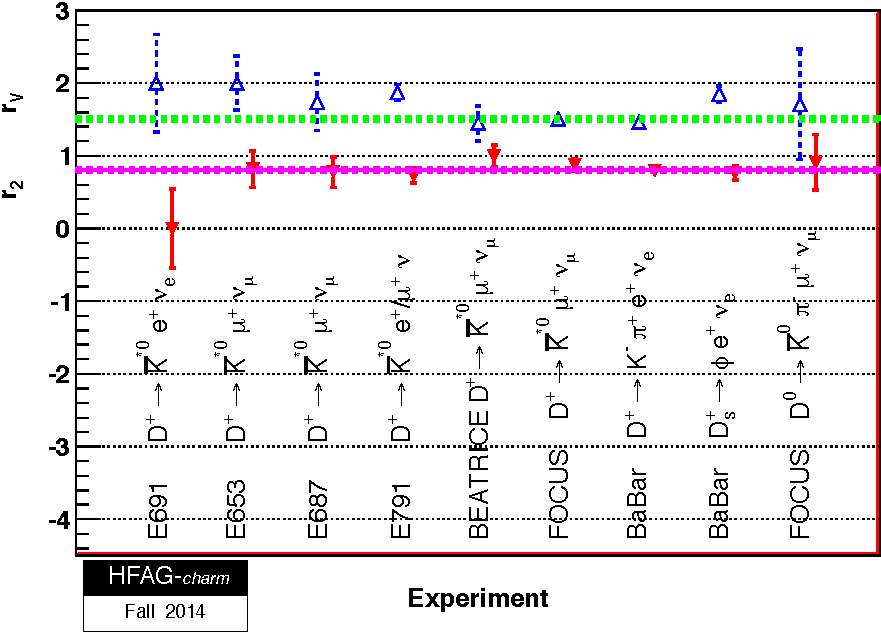
\includegraphics[width=6in,bb=0 0 550 400,angle=0]{figures/charm/sl_r2rv_hfag.pdf}
%    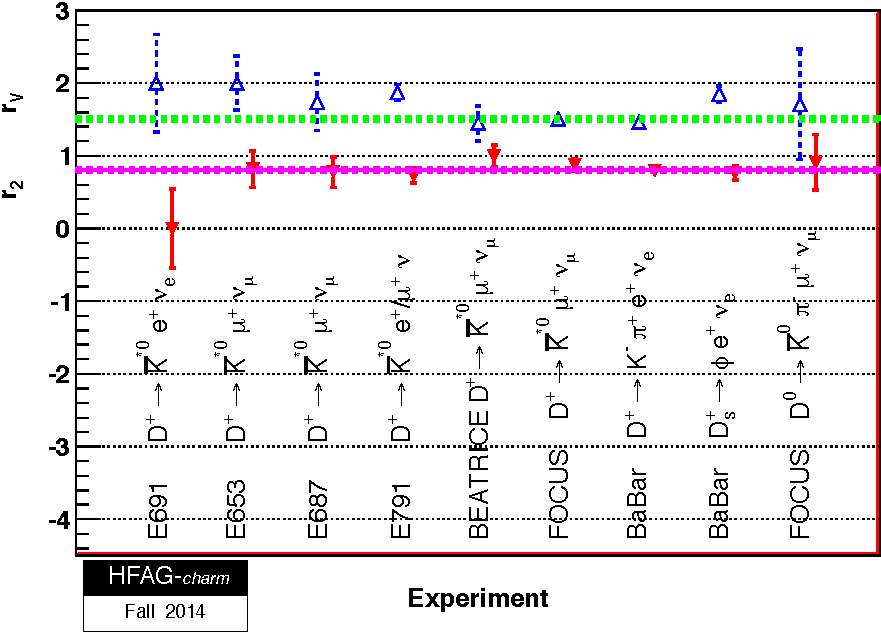
\includegraphics[width=6.5in,angle=0]{figures/charm/sl_r2rv_hfag.pdf}
  \end{center}
\vskip0.10in
  \caption{A comparison of $r_2$ and $r_V$ values 
    from various experiments. The first seven measurements are for $D^+
    \to K^-\pi^+ l^+\nu_l$ decays. Also shown as a line with
    1-$\sigma$ limits is the average of these. The last two points are
    $D_s^+$ decays and Cabibbo-suppressed $D$ decays. 
  \label{fig:r2rv}}
\end{figure}

\subsubsection{$S$-wave component}

In 2002 FOCUS reported~\cite{Link:2002ev} an asymmetry in
the observed $\cos(\theta_V)$ distribution. This is interpreted as
evidence for an $S$-wave component in the decay amplitude as follows. 
Since $H_0$ typically dominates over $H_{\pm}$, the distribution given 
by Eq.~(\ref{eq:dGammaVector}) is, after integration over $\chi$,
roughly proportional to $\cos^2\theta_V$. 
Inclusion of a constant $S$-wave amplitude of the form $A\,e^{i\delta}$ 
leads to an interference term proportional to 
$|A H_0 \sin\theta_\ell \cos\theta_V|$; this term causes an asymmetry 
in $\cos(\theta_V)$.
When FOCUS fit their data including this $S$-wave amplitude, 
they obtained $A = 0.330 \pm 0.022 \pm 0.015$ GeV$^{-1}$ and 
$\delta = 0.68 \pm 0.07 \pm 0.05$~\cite{Link:2002wg}. 

More recently, both \babar~\cite{Aubert:2008rs} and 
CLEO-c~\cite{Ecklund:2009fia} have also found evidence 
for an $f^{}_0$ component in semileptonic $D^{}_s$ decays.



\subsubsection{Model-independent form factor measurement}

Subsequently the CLEO-c collaboration extracted the form factors
$H_+(q^2)$, $H_-(q^2)$, and $H_0(q^2)$ in a model-independent fashion
directly as functions of $q^2$~\cite{Briere:2010zc} and also determined the
$S$-wave form factor $h_0(q^2)$ via the interference term, despite the
fact that the $K\pi$ mass distribution appears dominated by the vector
$K^*(892)$ state. Their results are shown in Figs.~\ref{fig:cleoc_H} and
\ref{fig:cleoc_h0}.  Plots in Fig.~\ref{fig:cleoc_H} clearly show that
$H_0(q^2)$ dominates over essentially the full range of $q^2$, but
especially at low $q^2$. They also show that the transverse form factor
$H_t(q^2)$ (which can be related to $A_3(q^2)$ is small (compared to
Lattice Gauge Theory calculations) and suggest that the form factor
ratio $r_3 \equiv A_3(0) / A_1(0)$ is large and negative.

The product $H_0(q^2)\times h_0(q^2)$ is shown in
Fig.~\ref{fig:cleoc_h0} and clearly indicates the existence of
$h_0(q^2)$, although it seems to fall faster with $q^2$ than $H_0(q^2)$.
The other plots in that figure show that $D$- and $F$-wave versions of
the $S$-wave $h_0(q^2)$ are not significant.

\begin{figure}[htb]
  \begin{center}
    \vskip0.20in
    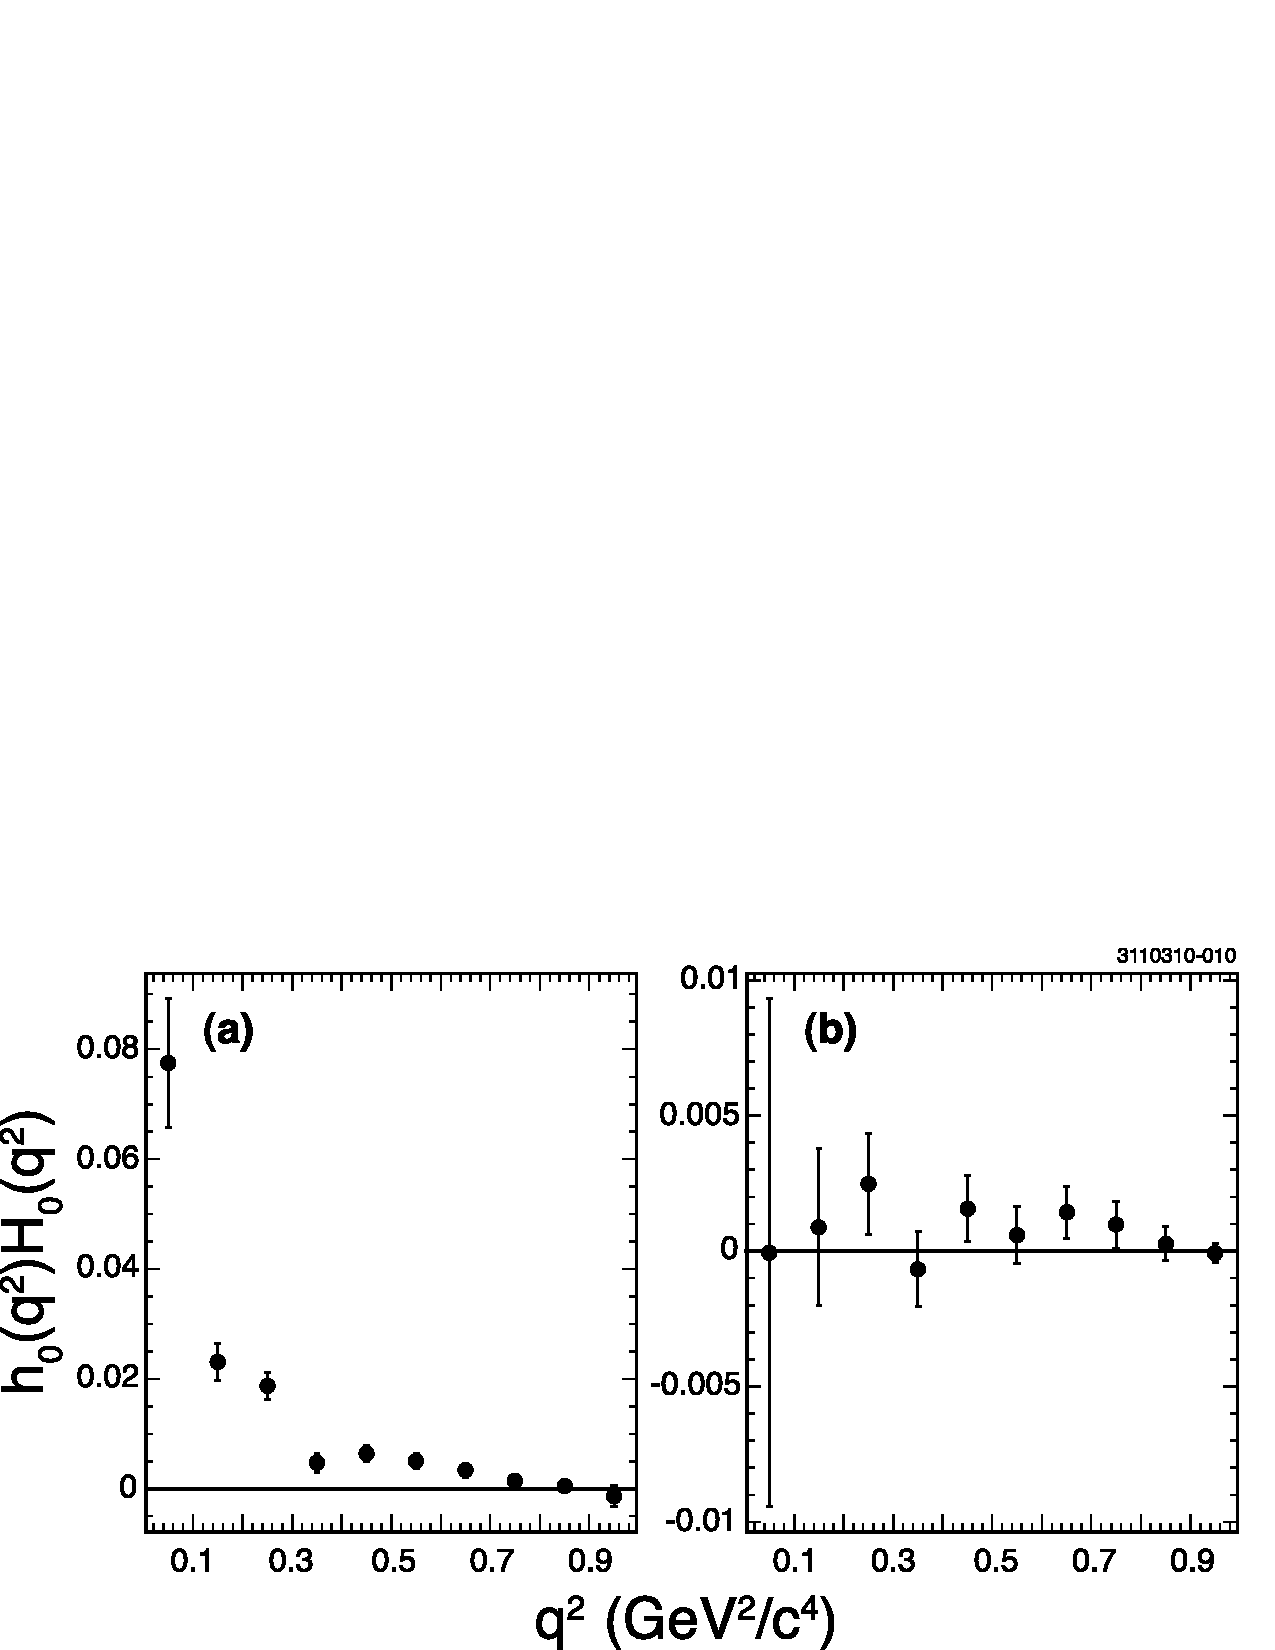
\includegraphics[width=4.in,angle=0., bb= -3 -3 598 330]{figures/charm/sl_cleoc_h0.pdf}
  \end{center}
  \begin{center}
    \vskip0.20in
    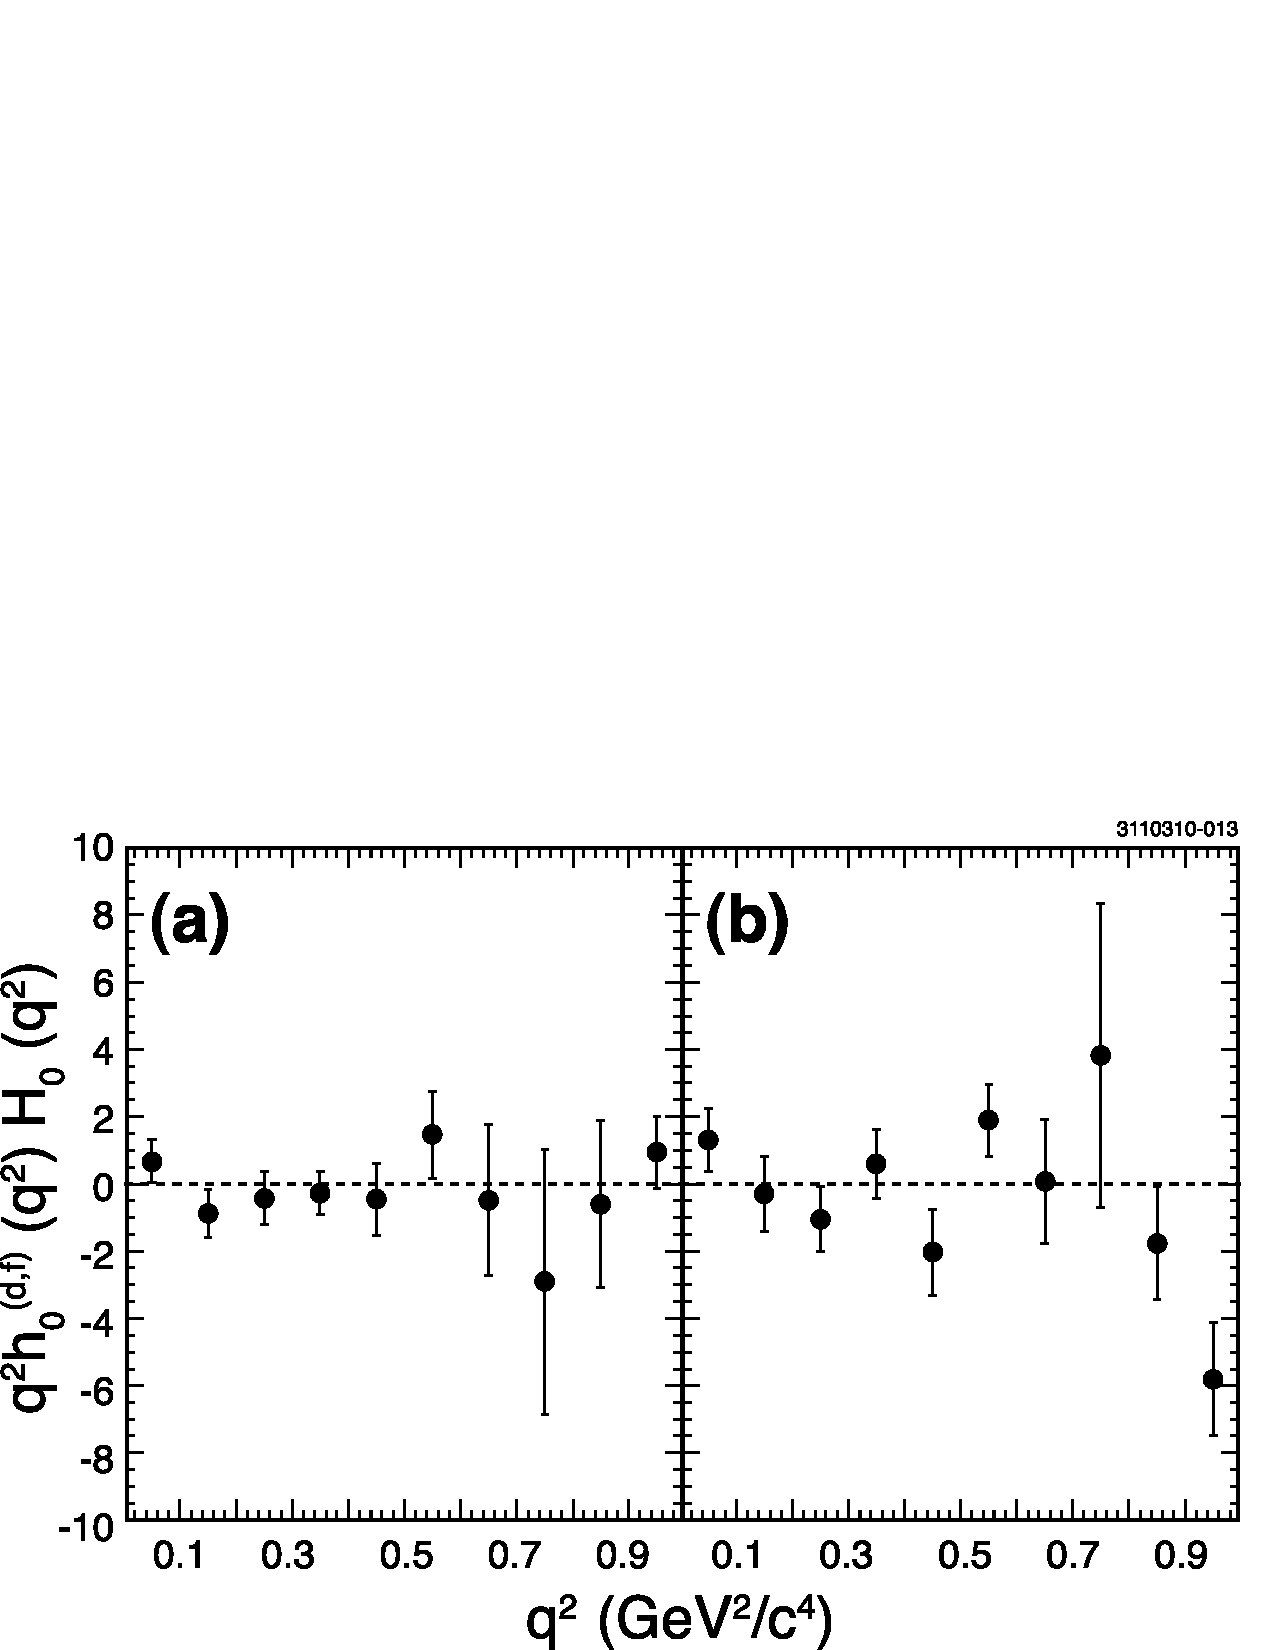
\includegraphics[width=4.in,angle=0., bb= -3 -3 598 390]{figures/charm/sl_cleoc_h0df.pdf}
  \end{center}
\vskip-0.20in
  \caption{Model-independent form factors $h_0(q^2)$ measured by 
    CLEO-c~\cite{Briere:2010zc}.
  \label{fig:cleoc_h0}}
\end{figure}

\begin{figure}[htb]
  \begin{center}
    \vskip0.20in
    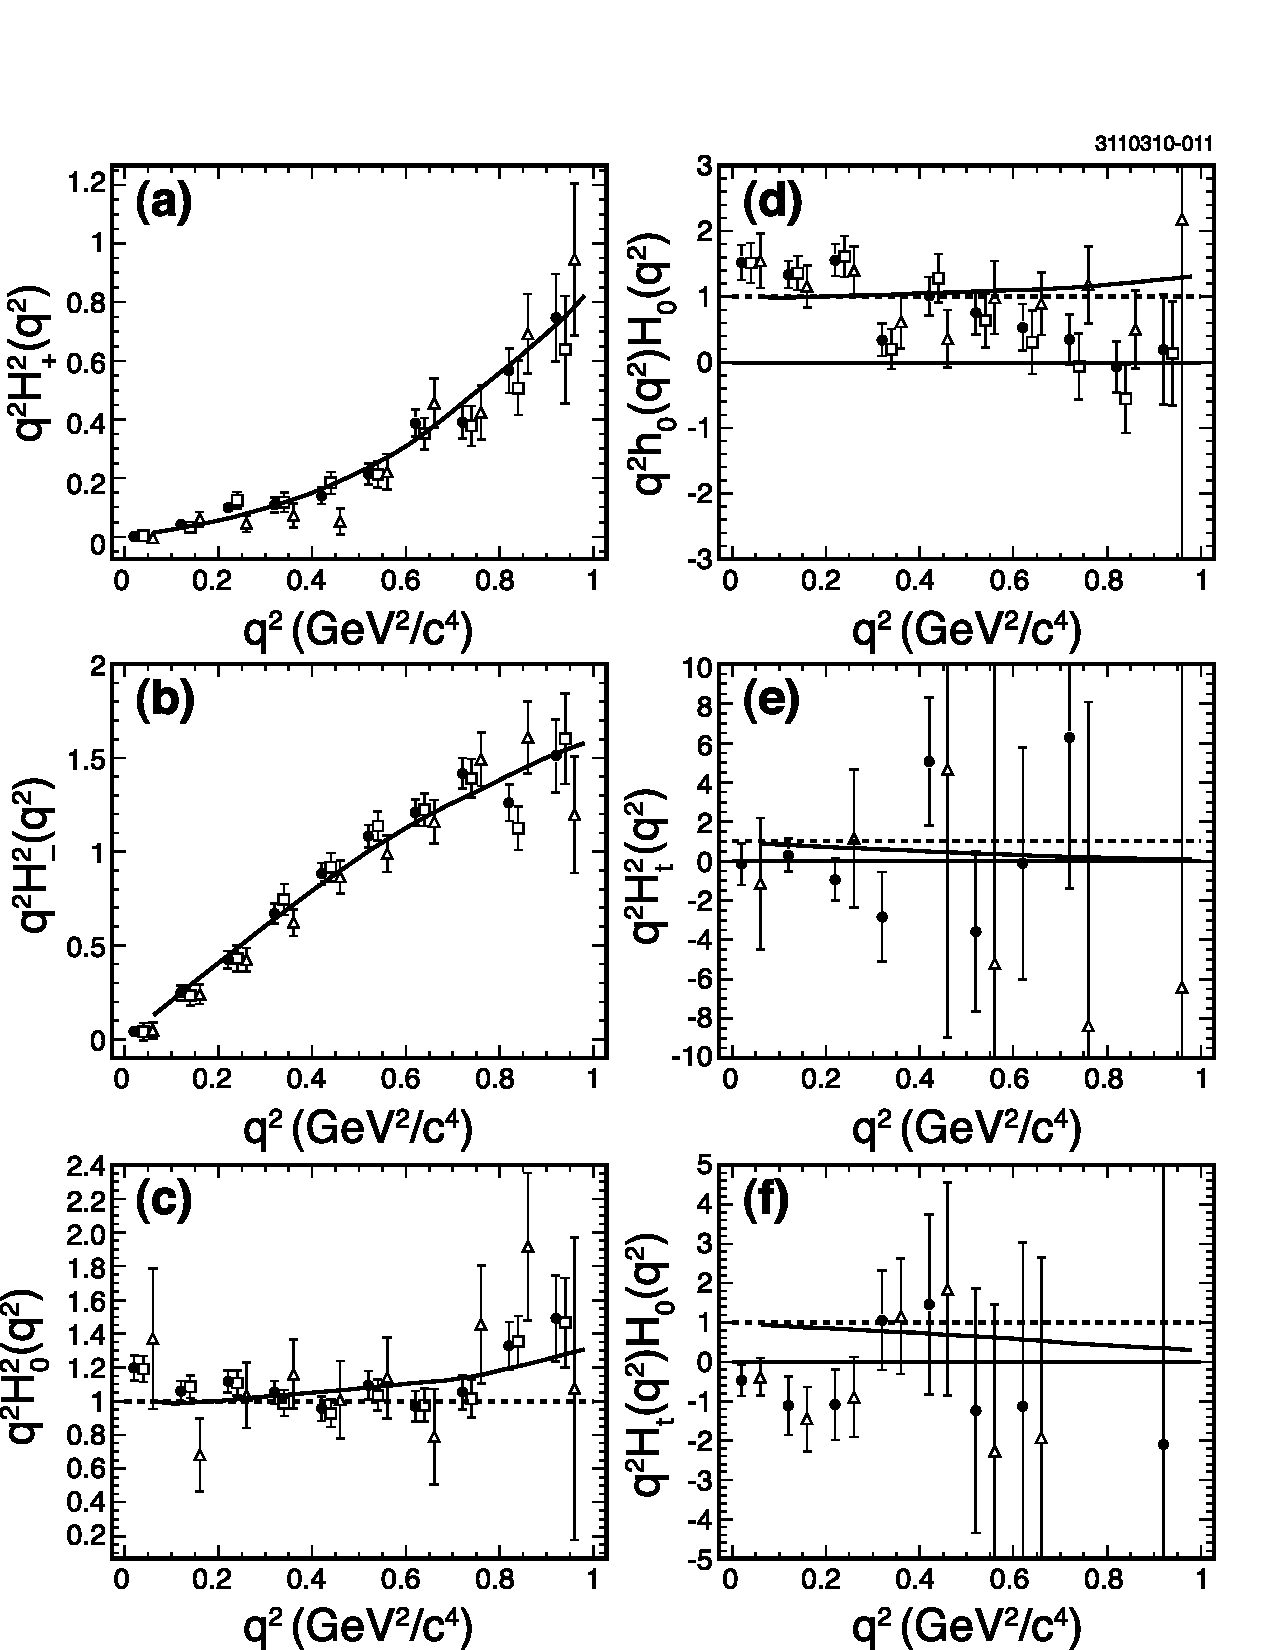
\includegraphics[width=4.in,angle=0., bb= -3 -3 595 720]{figures/charm/sl_cleoc_H.pdf}
  \end{center}
\vskip-0.20in
  \caption{Model-independent form factors $H(q^2)$ measured by 
    CLEO-c~\cite{Briere:2010zc}.
  \label{fig:cleoc_H}}
\end{figure}

\subsubsection{Detailed measurements of the $D^+ \rightarrow K^- \pi^+ e^+ \nu_e$ 
decay channel}

\babar \cite{delAmoSanchez:2010fd} has selected a large sample of $244\times 10^3$ signal events with a ratio $S/B\sim 2.3$ from an analyzed integrated
luminosity of $347~\fb^{-1}$. With four particles emitted in the final state, 
the differential decay rate depends on five variables.
In addition to the four variables defined in previous sections there is 
$m^2$, the mass squared of the $K\pi$ system.
Apart from this last variable, the reconstruction algorithm does not provide 
a high resolution on the other measured quantities 
%(see the similar measurement of the $D^0 \rightarrow K^- e^+ \nu_e$ decay channel)
and a multi-dimensional unfolding procedure
is not used to correct for efficiency and resolution effects. Meanwhile these
limitations still allow an essentially model independent measurement of
the differential decay rate. This is because, apart from the $q^2$
and mass dependence of the form factors, angular distributions are fixed by
kinematics. In addition, present accurate measurements of 
$D \rightarrow P \overline{\ell}\nu_{\ell}$ decays have shown that the 
$q^2$ dependence of the form factors can be well described by several models
as long as the corresponding model parameter(s) are fitted on data.
This is even more true in $D \rightarrow V \overline{\ell}\nu_{\ell}$ decays
because the $q^2$ range is reduced. To analyze the
$D^+ \rightarrow K^- \pi^+ e^+ \nu_e$ decay channel it is assumed
that all form factors have a $q^2$ variation given by
the simple pole model and the effective pole mass value,
 $m_A=(2.63 \pm 0.10 \pm 0.13)~GeV/c^2$,
is fitted
for the axial vector form factors. This value is compatible
with expectations when comparing with the mass
of $J^P=1^+$ charm mesons. Data are not sensitive to the effective mass
of the vector form factor for which $m_V=(2.1 \pm 0.1)~GeV/c^2$ is used,
nor to the effective pole mass of the scalar component for which $m_A$ is used.
 For the mass dependence of the form factors,
a Breit-Wigner with a mass dependent width and a Blatt-Weisskopf damping factor
is used. For the S-wave amplitude, considering
what was measured in $D^+ \rightarrow K^- \pi^+\pi^+$ decays,
a polynomial variation below the $\overline{K}^*_0(1430)$
and a Breit-Wigner distribution, above are assumed. For the polynomial part, 
a linear term is sufficient to fit data.

It is verified that the variation of the S-wave phase is compatible 
with expectations from elastic $K\pi$ scattering, according
to the Watson theorem. At variance with elastic scattering, 
a negative relative sign between the S- and P-waves is measured; 
this is compatible with 
the previous theorem. In Fig. \ref{fig:swave_phase}, the measured
S-wave phase is compared with the phase of the elastic, $I=1/2$,
$K\pi$ elastic phase for different values of the $K\pi$ mass.

\begin{figure}[!htb]
	\centering
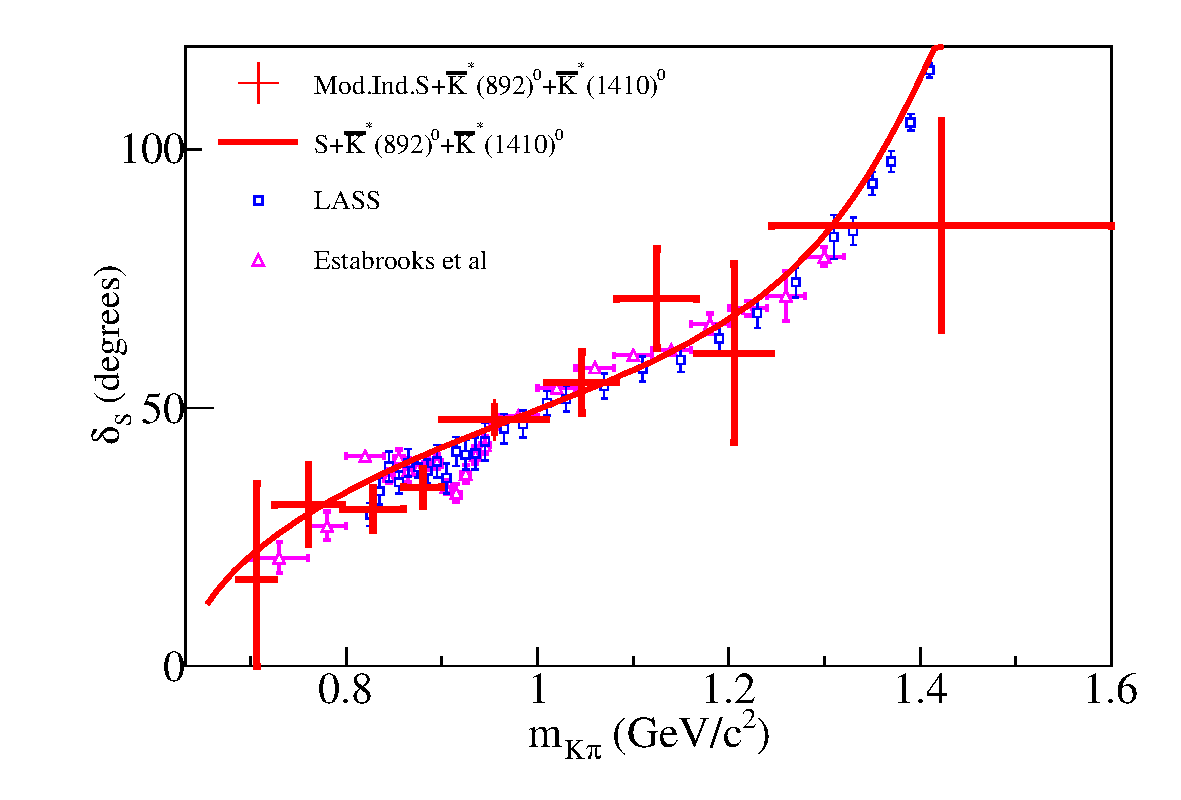
\includegraphics[bb=0 0 567 384, width=0.6\textwidth]{figures/charm/sl_babar_swave_hfag2012.pdf}
\caption{Points (full circles) give the \babar $S$-wave phase variation 
assuming a signal containing $S$-wave, $\akst$ and $\akstp$ components. 
Error bars include systematic uncertainties.
The full line corresponds to a parameterized $S$-wave phase variation 
fitted on \babar data.
The phase variation measured in $K\pi$ scattering
by Ref. \cite{Estabrooks:1977xe} (triangles) and LASS \cite{Aston:1987ir} (squares), 
after correcting 
for $\delta^{3/2}$, are given.}
\label{fig:swave_phase}
\end{figure}

Contributions from other resonances decaying into $K^-\pi^+$ are considered.
A small signal from the $\overline{K}^*(1410)$ is observed, compatible
with expectations from $\tau$ decays and this component is included in the
nominal fit. In total, 11 parameters are fitted in addition to the total
number of signal events. They give a detailed description of the differential
decay rate versus the 5 variables and corresponding matrices for 
statistical and systematic uncertainties are provided allowing to 
evaluate the compatibility of data with future theoretical expectations.

In Fig. \ref{fig:h0FF}, measured values from CLEO-c
of the products $q^2H_0^2(q^2)$ and $q^2h_0(q^2)H_0(q^2)$ are compared with 
corresponding results from \babar illustrating the difference in behavior
of the scalar $h_0$ component and the helicity zero $H_0$ P-wave form factor.
For this comparison, the plotted values from \babar for the two distributions
are fixed to 1 at $q^2=0$. The different behavior of $h_0(q^2)$
and $H_0(q^2)$ can be explained by they different dependence in the 
$p^*$ variable.
\begin{figure}[htbp!]
  \begin{center}
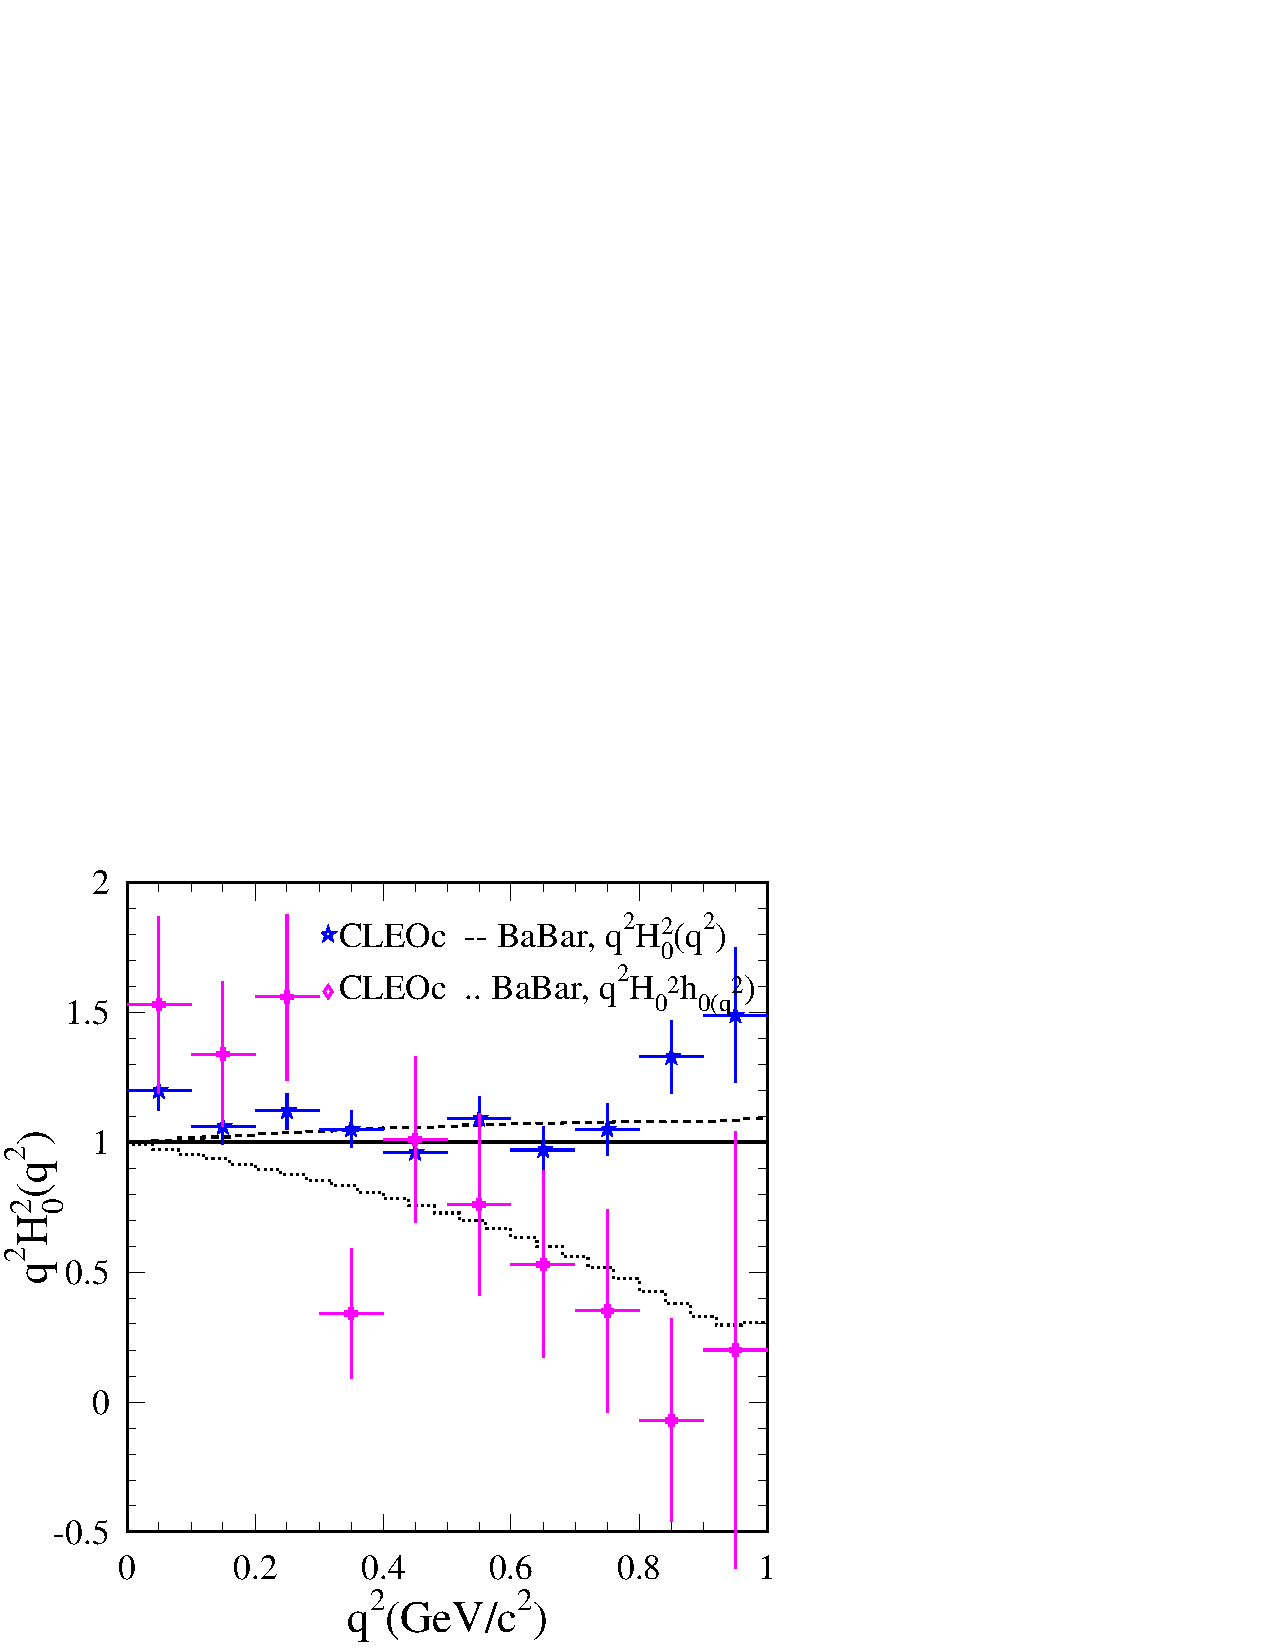
\includegraphics[bb=0 0 425 425,width=.60\textwidth]{figures/charm/sl_ff_compar_cleoc.pdf}
  \end{center}
  \caption[]{{Comparison between CLEO-c measurements and \babar results
for the quantities $q^2H_0^2(q^2)$ and
 $q^2H_0(q^2)h_0(q^2)$.}
   \label{fig:h0FF}}
\end{figure}
Results of this analysis for the rates and few characteristics 
for S, P and D-waves are given in Table \ref{tab:comparison}.

\begin{table}[!htb]
\begin{center}
 \caption[]{{Detailed determination of the properties of the 
$D^+ \rightarrow K^-\pi^+ e^+ \nu_e$ decay channel from \babar. 
Values for ${\cal B}(D^+\rightarrow \akstp / \akstd e^+\nu_e)$ are corrected for their respectivebranching fractions into $K^-\pi^+$.}\hspace{1cm}
  \label{tab:comparison}}
\begin{tabular}{c c}
\vspace*{-10pt} & \\
\hline
\textbf{Measurement} & \textbf{\babar result} \\
\hline\hline
{ $m_{\kst}(~MeV/c^2)$} & {$895.4\pm{0.2}\pm0.2$}\\
{ $\Gamma^0_{\kst}(~MeV/c^2)$} & {$46.5\pm{0.3}\pm0.2$} \\
{$r_{BW}(~GeV/c)^{-1}$ }& {$2.1\pm{0.5}\pm 0.5$} \\
\hline
{$r_{V}$} & {$1.463\pm{0.017}\pm 0.031$} \\
{$r_{2}$} & {$0.801\pm{0.020}\pm 0.020$}  \\
{ $m_{A} (~GeV/c^2)$} & {$2.63\pm 0.10 \pm 0.13$}\\
\hline
${\cal B}(D^+ \rightarrow K^-\pi^+ e^+ \nu_e)(\%)$ &$4.04 \pm 0.03 \pm 0.04 \pm 0.09$ \\
${\cal B}(D^{+}\rightarrow K^- \pi^+ e^{+} \nu_{e})_{\overline{K}^{*0}}(\%)$ & $3.80\pm0.04\pm0.05 \pm0.09 $  \\ 
${\cal B}(D^+ \rightarrow K^-\pi^+ e^+ \nu_e)_{S-wave}(\%)$ &$0.234 \pm0.007  \pm0.007  \pm0.005  $ \\
${\cal B}(D^{+}\rightarrow \akstp e^{+} \nu_{e})(\%)$ & $0.30\pm0.12\pm0.18\pm0.06$ ($<0.6$ at 90$\%$ C.L.) \\ 
${\cal B}(D^{+}\rightarrow \akstd e^{+} \nu_{e})(\%)$ & $0.023\pm0.011\pm0.011\pm0.001$ ($<0.05$ at 90$\%$ C.L.)  \\ 
\hline\hline
\end{tabular}
\end{center}
\end{table}

%%%%%%%%%%%%%%%%%%%%%%%%%%%%%%%%%%%%%%%%%%%%%%%%%%%%%%
